%! TEX program = LuaTeX

\documentclass[nobackground,dvipsnames,table,aspectratio=169]{beamer}
\usepackage{cs152}

\mode<presentation>
{\usetheme{Hannover}
    \usecolortheme{cs152}
    \setbeamercovered{transparent}
    \useinnertheme[shadow=false]{rounded}
    \usebackgroundtemplate{}
    \setbeamercolor*{frametitle}{parent=palette primary}
    \setbeamerfont{block title}{size={}}
    \setbeamertemplate{navigation symbols}{}
}

\title{Misinformation and Disinformation}
\subtitle{CS 152 --- Lecture 11}

\author[A. Stamos]{Alex Stamos}
\institute[Stanford University]{Stanford Cyber Policy Center}
\date[2022]{\today}
\subject{CS 152 --- Trust and Safety Engineering}
%\titlegraphic{
\includegraphics[width=5cm]{img/cyber-logo-white-black-red-WEB}}

% Change the level of bulleting on the ToC page
\setcounter{tocdepth}{2}

\graphicspath{{img/lesson11}}

\begin{document}

\begin{frame}
    \titlepage
\end{frame}

\begin{frame}{Dr. Mohamed Shafi}
    \begin{columns}
        \column{0.4\textwidth}
            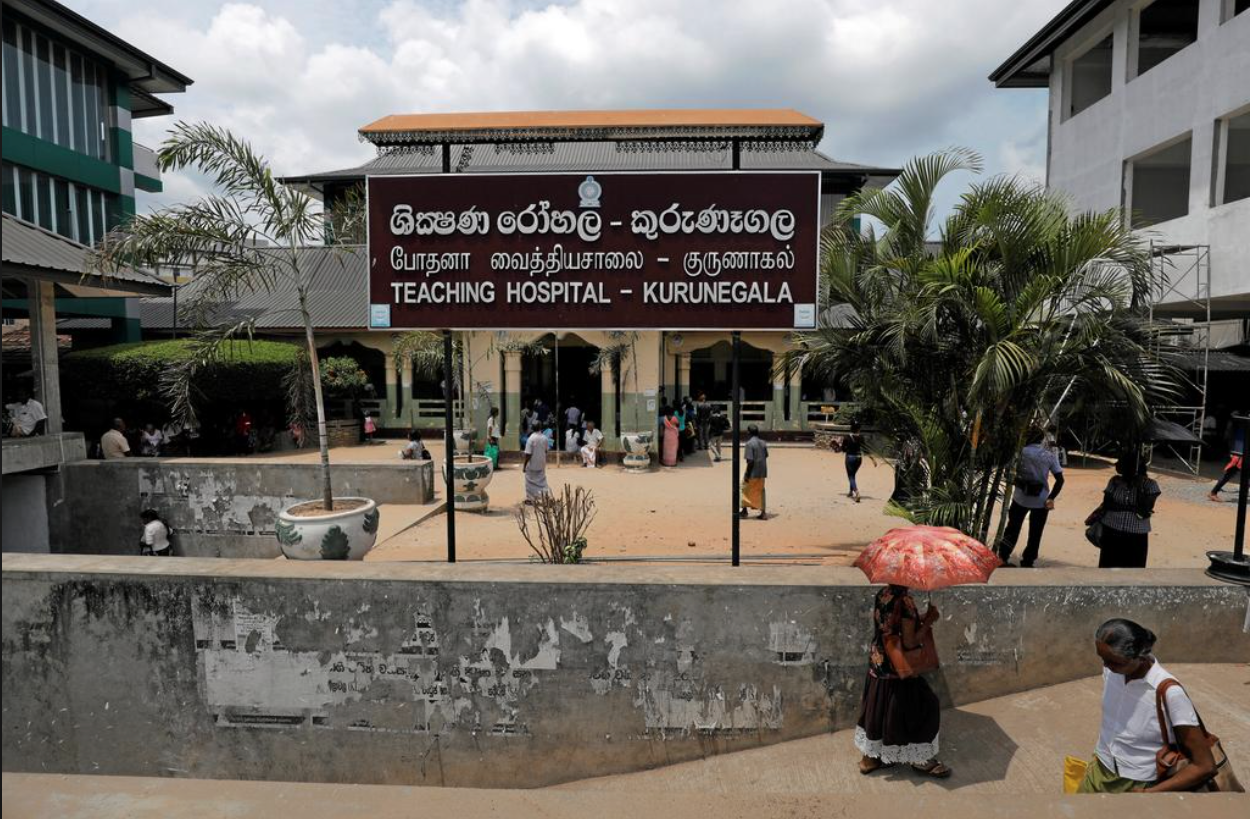
\includegraphics[width=0.9\textwidth]{dr-shafi-1}
            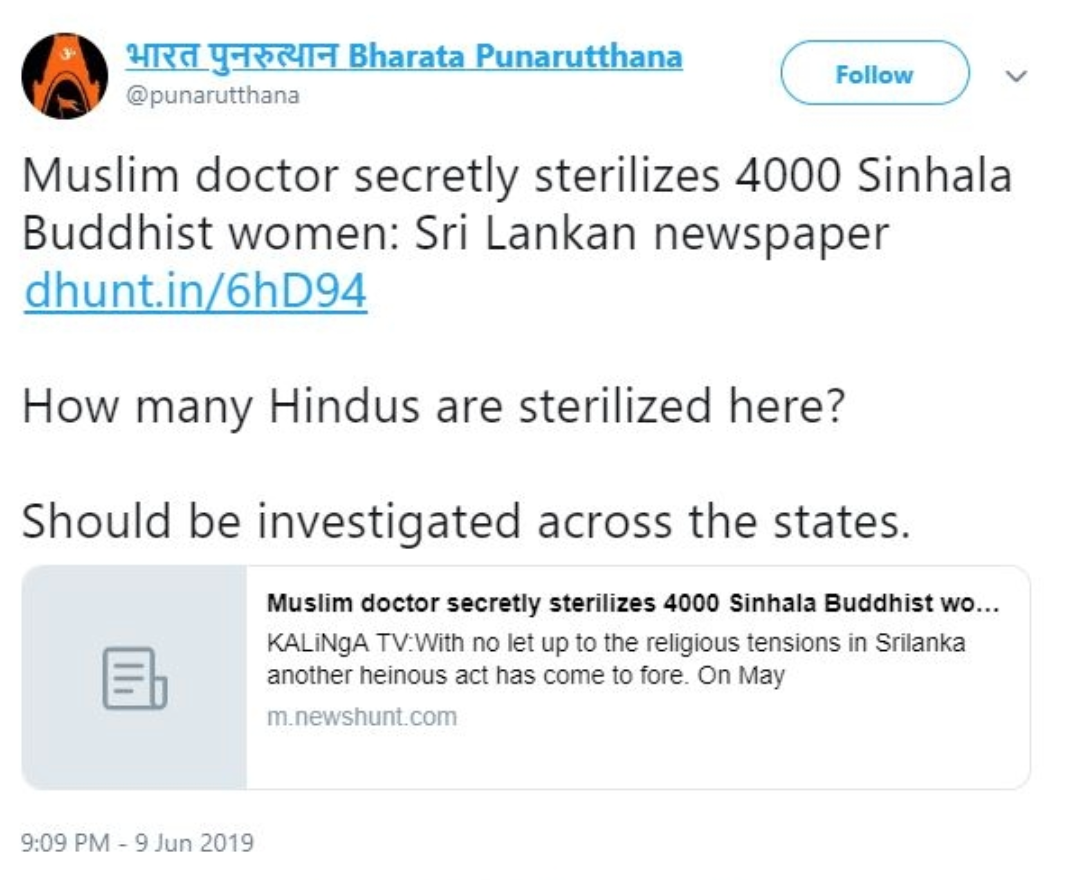
\includegraphics[width=\textwidth]{dr-shafi-2}
        \column{0.6\textwidth}
            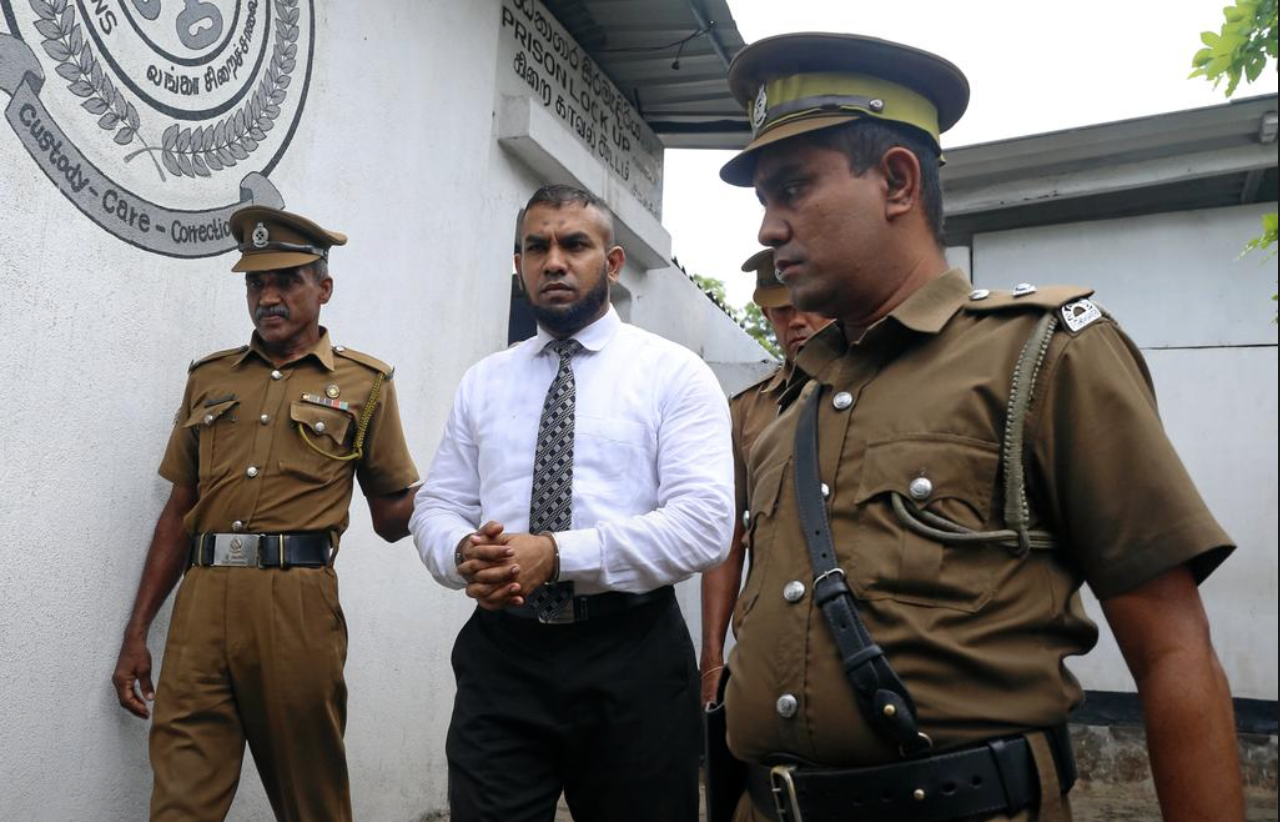
\includegraphics[width=\textwidth]{dr-shafi-3}
    \end{columns}
\end{frame}

\section{What Will We Learn Today?}

\begin{frame}{What Will We Learn Today?}
    \large
    \begin{itemize}
        \item Definitions, actors, and goals
        \item Forms of online narrative laundering
        \item How the current information environment and ecosystem is the same as, and different from, the past.
        \item What disinformation franchising looks like
        \item Novel disinformation tactics
        \item What commercially motivated disinformation looks like
        \item How technological changes have impacted information integrity
        \item What can we do about this?
    \end{itemize}
\end{frame}

\section{Understanding Mis/Disinformation}

\begin{frame}{Definitions}
    \textbf{Misinformation}: Unintentionally inaccurate information\\~\\
    
    \textbf{Two distinct definitions of disinformation:}
    \begin{enumerate}
        \item Deliberately false or misleading information
        \item Information with the intent to deceive (information can be false, but need not be false, the deception can come from the behavior, like having a fake account)
    \end{enumerate}
    
    \textbf{Political Propaganda}: Information used to promote a particular political cause or point of view (could be misleading, but could be true; old tactic)\\~\\
    
    \textbf{“Fake News”:} News stories that are false – this is not a term that researchers use\\~\\
    
    \textbf{*Meanings overlap and word choice can be a matter of perspective}
\end{frame}

\begin{frame}{Is This Disinformation?}
    \centering
    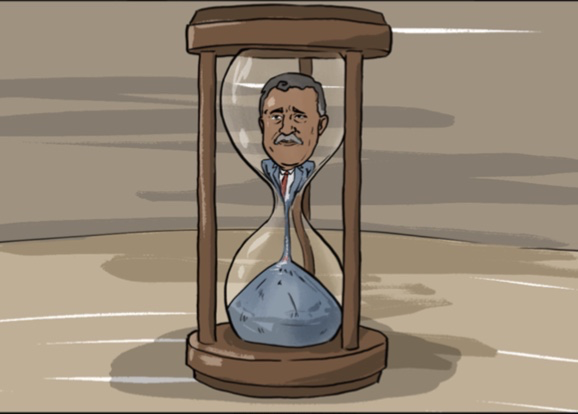
\includegraphics[width=0.6\textwidth]{is-this-disinfo}
\end{frame}

\begin{frame}{Understanding Motivations}
    \begin{columns}
        \column{0.3\textwidth}
            \underline{Actors}
            \begin{itemize}
                \item Nation states
                \item Terrorist organizations
                \item Domestic ideologues
                \item Mercenaries
                \item Spammers
                \item Trolling factories
            \end{itemize}
        \column{0.7\textwidth}
            \centering
            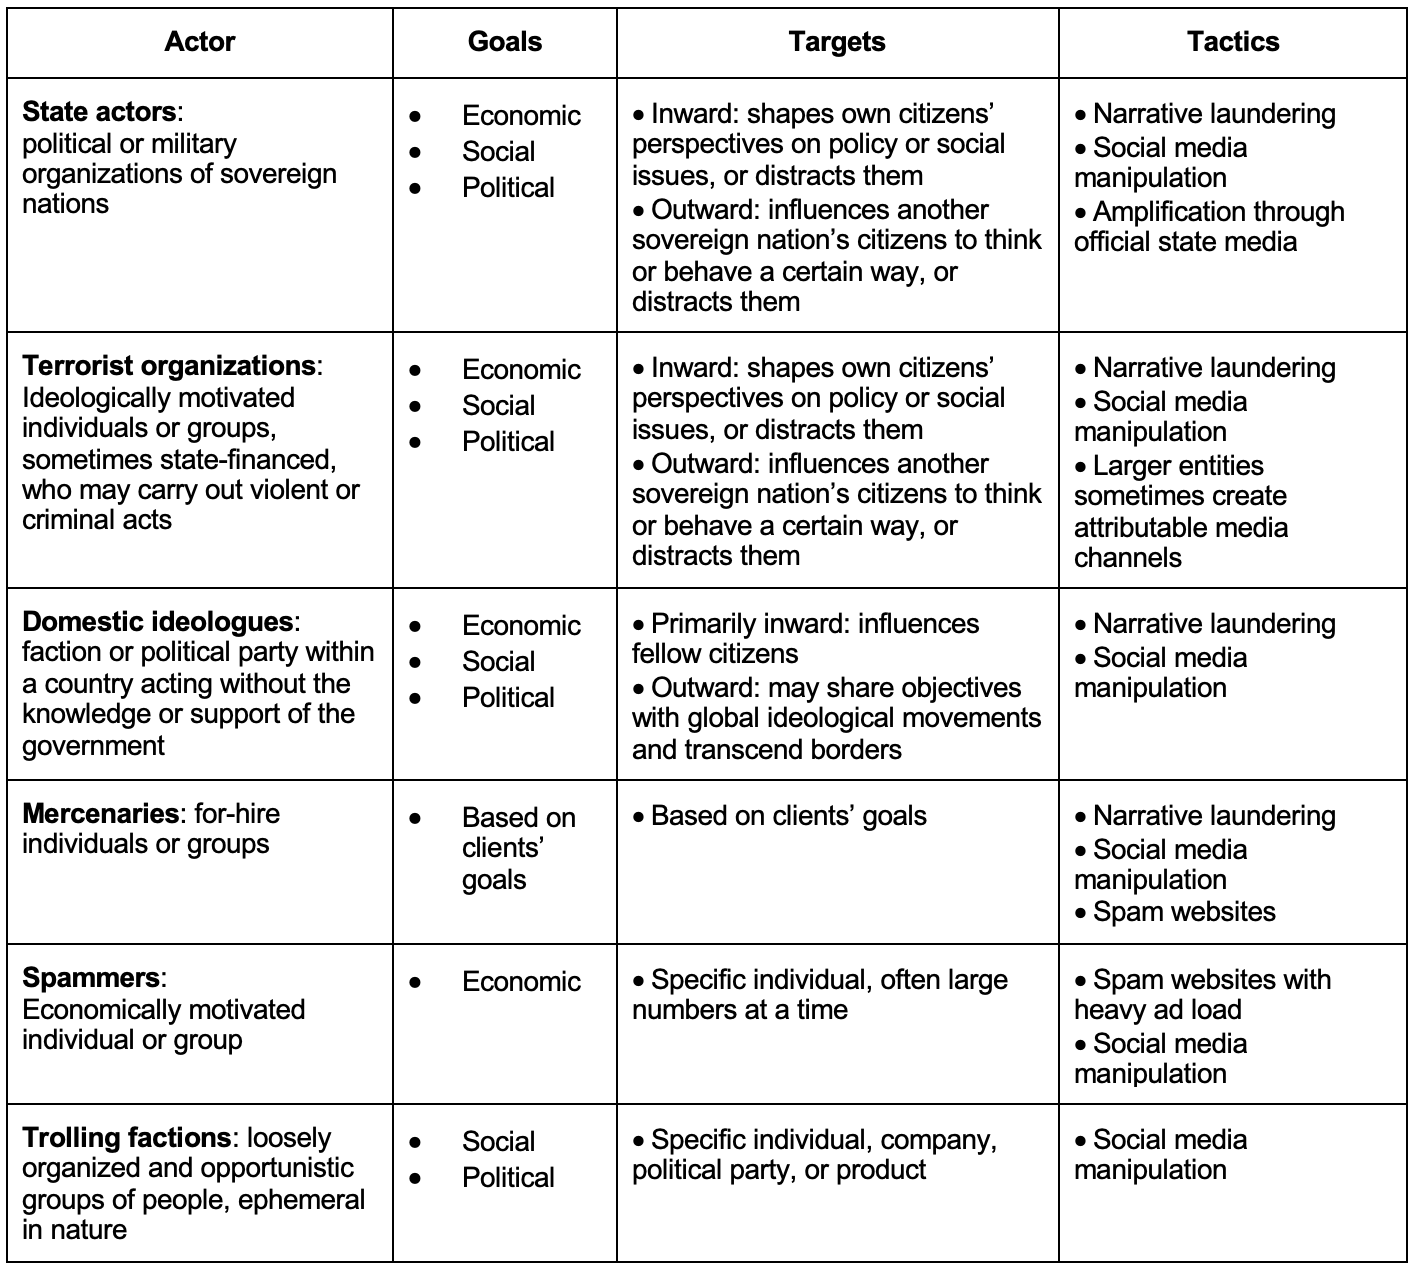
\includegraphics[height=0.856\textheight]{actor-table}
    \end{columns}
\end{frame}

\begin{frame}{Major State Actors}
    \begin{columns}
        \column{0.2\textwidth}
            \begin{itemize}
                \item China
                \item Russia
                \item Iran
                \item U.S.
                \item Saudi Arabia
            \end{itemize}
        \column{0.8\textwidth}
            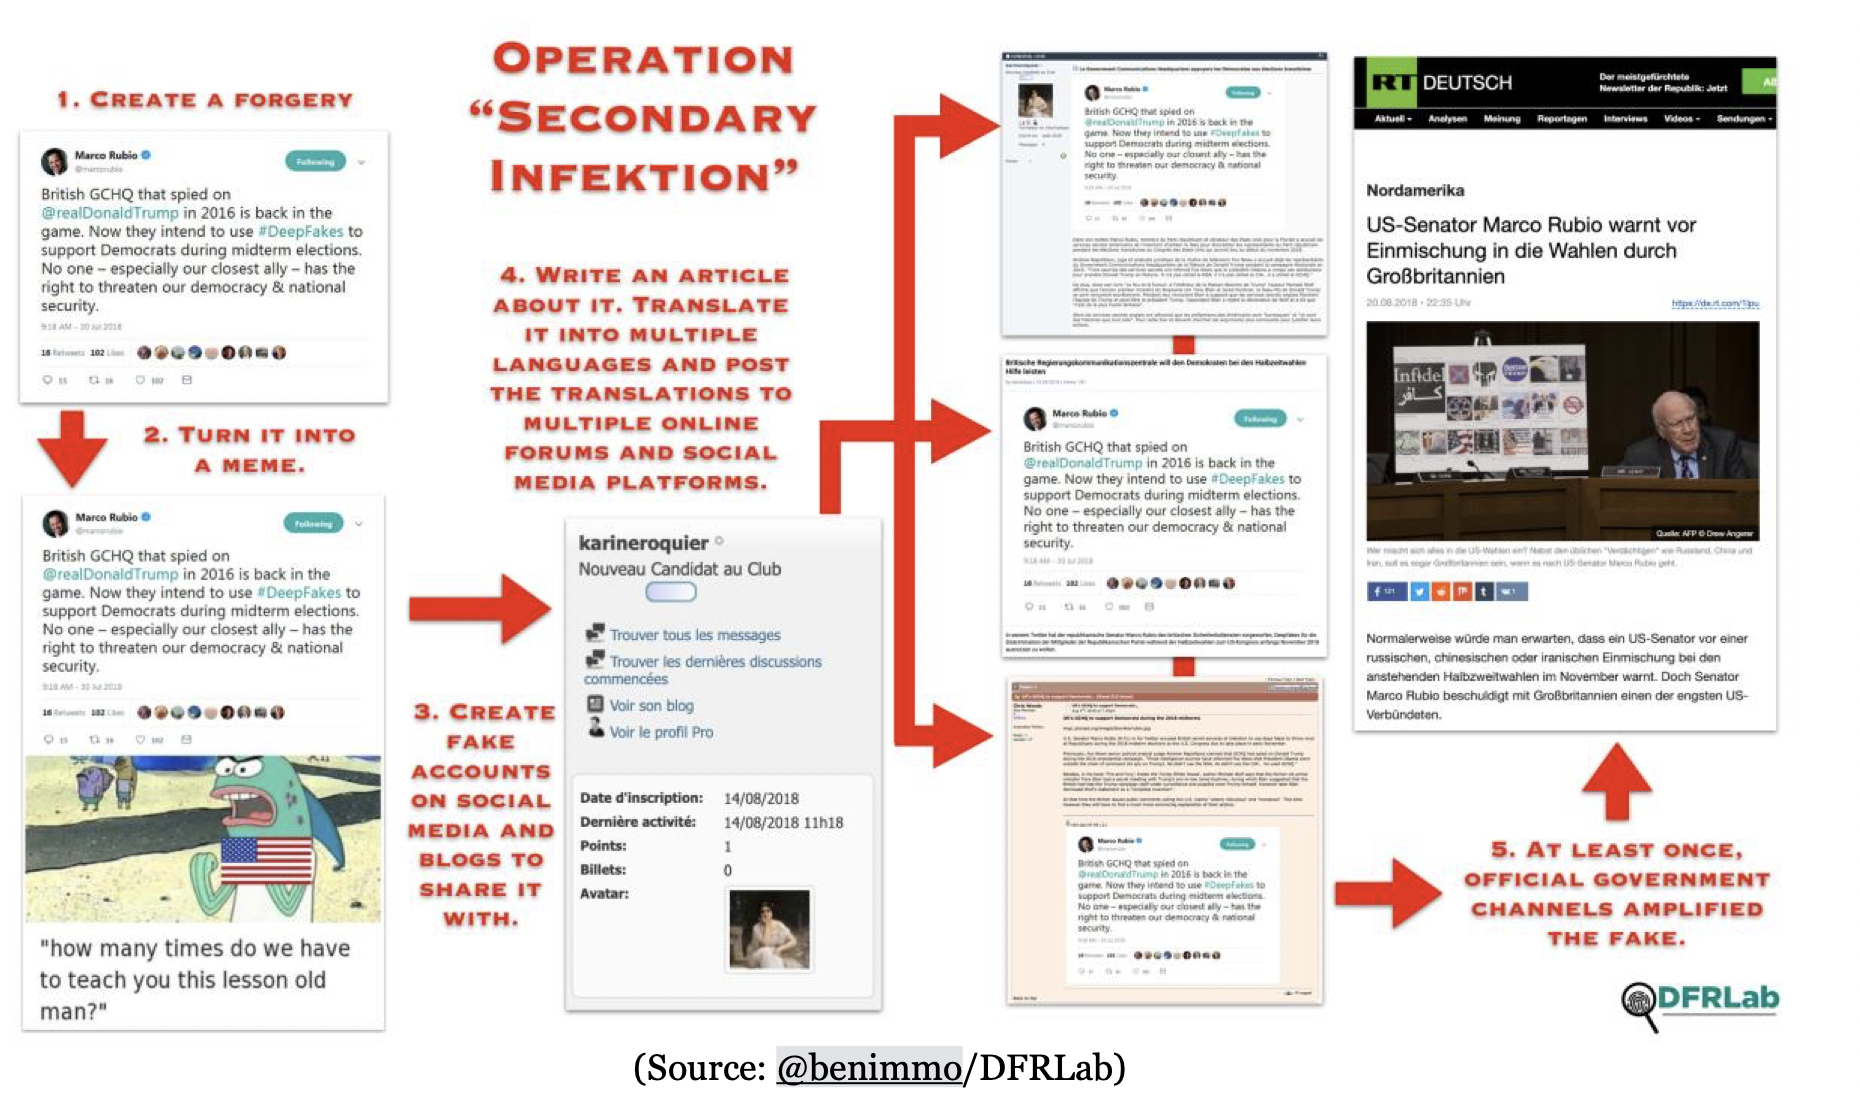
\includegraphics[width=\textwidth]{operation-secondary-infektion}
    \end{columns}
\end{frame}

\begin{frame}{Understanding Motivations}
    \underline{Goals}
    \begin{itemize}
        \item Own share of voice on a topic or within a hashtag
        \item Flood the zone, making it impossible to understand nuance or truth around an incident or narrative
        \item Infiltrate or develop deeper relationships with targeted communities to nudge them in a particular direction
        \item Sow social division
        \item Send audiences to a website owned by the actor (for monetization or future targeting)
        \item Persuade people toward a point of view
    \end{itemize}
\end{frame}

\begin{frame}{What Causes Misinformation to Spread?}
    \begin{columns}
        \column{0.4\textwidth}
            \begin{itemize}
                \item Distrust in authority
                \item Amateur participation
                \item Virality and automation
                \item Cross-platform spread
            \end{itemize}
        \column{0.6\textwidth}
            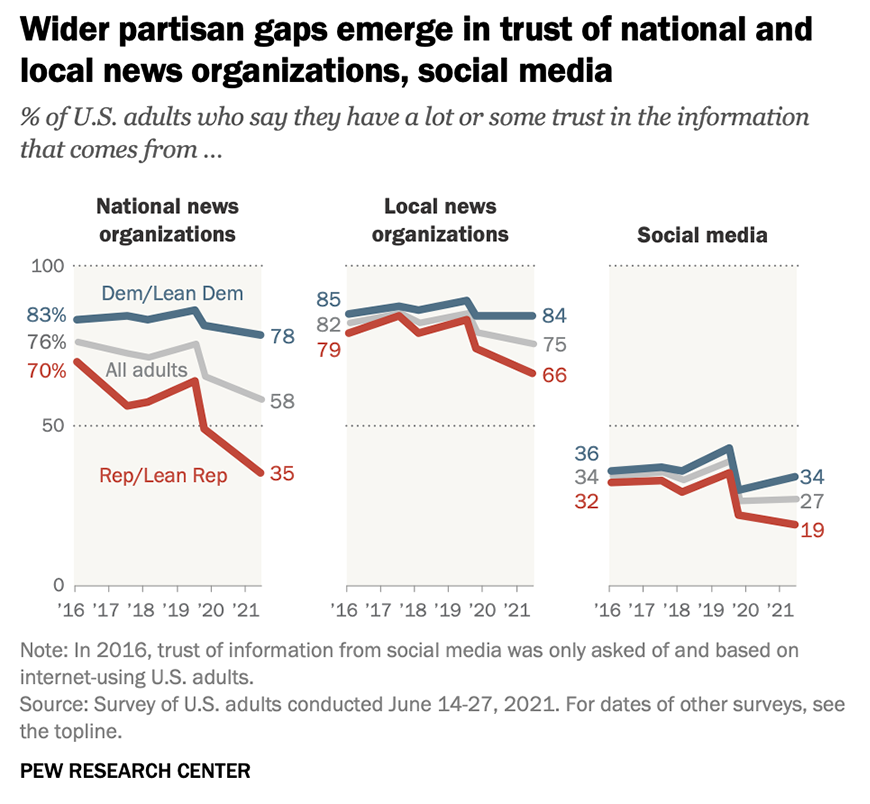
\includegraphics[width=\textwidth]{partisan-trust-gap}
    \end{columns}
\end{frame}

\begin{frame}{Government-Sponsored Disinformation}
    \centering
    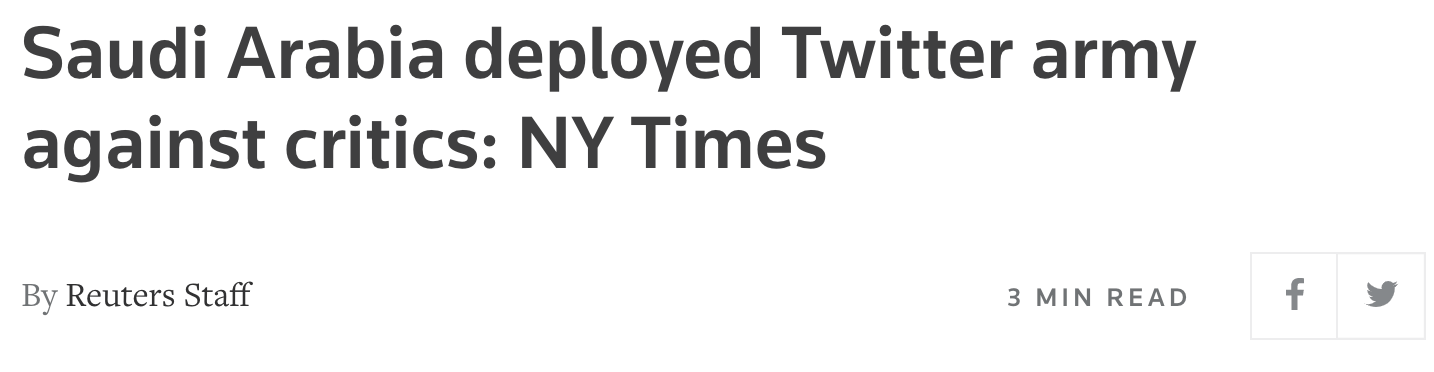
\includegraphics[width=0.6\textwidth]{govt-sponsored-disinfo-1}
    \begin{columns}
        \column{0.5\textwidth}
            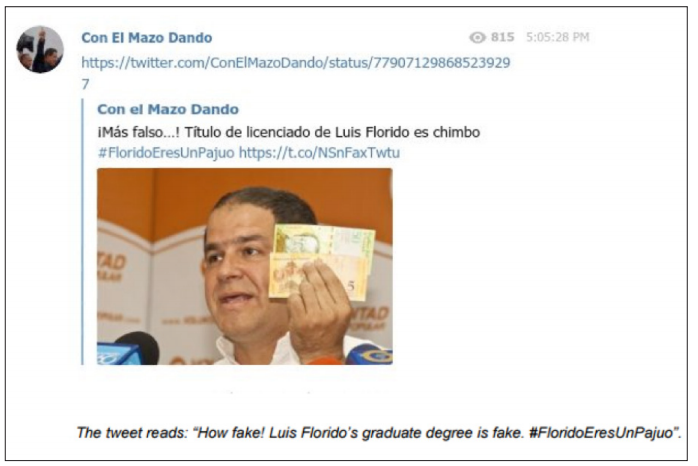
\includegraphics[width=\textwidth]{govt-sponsored-disinfo-2}
            \tiny
            State-directed trolling in Venezuela
        \column{0.5\textwidth}
            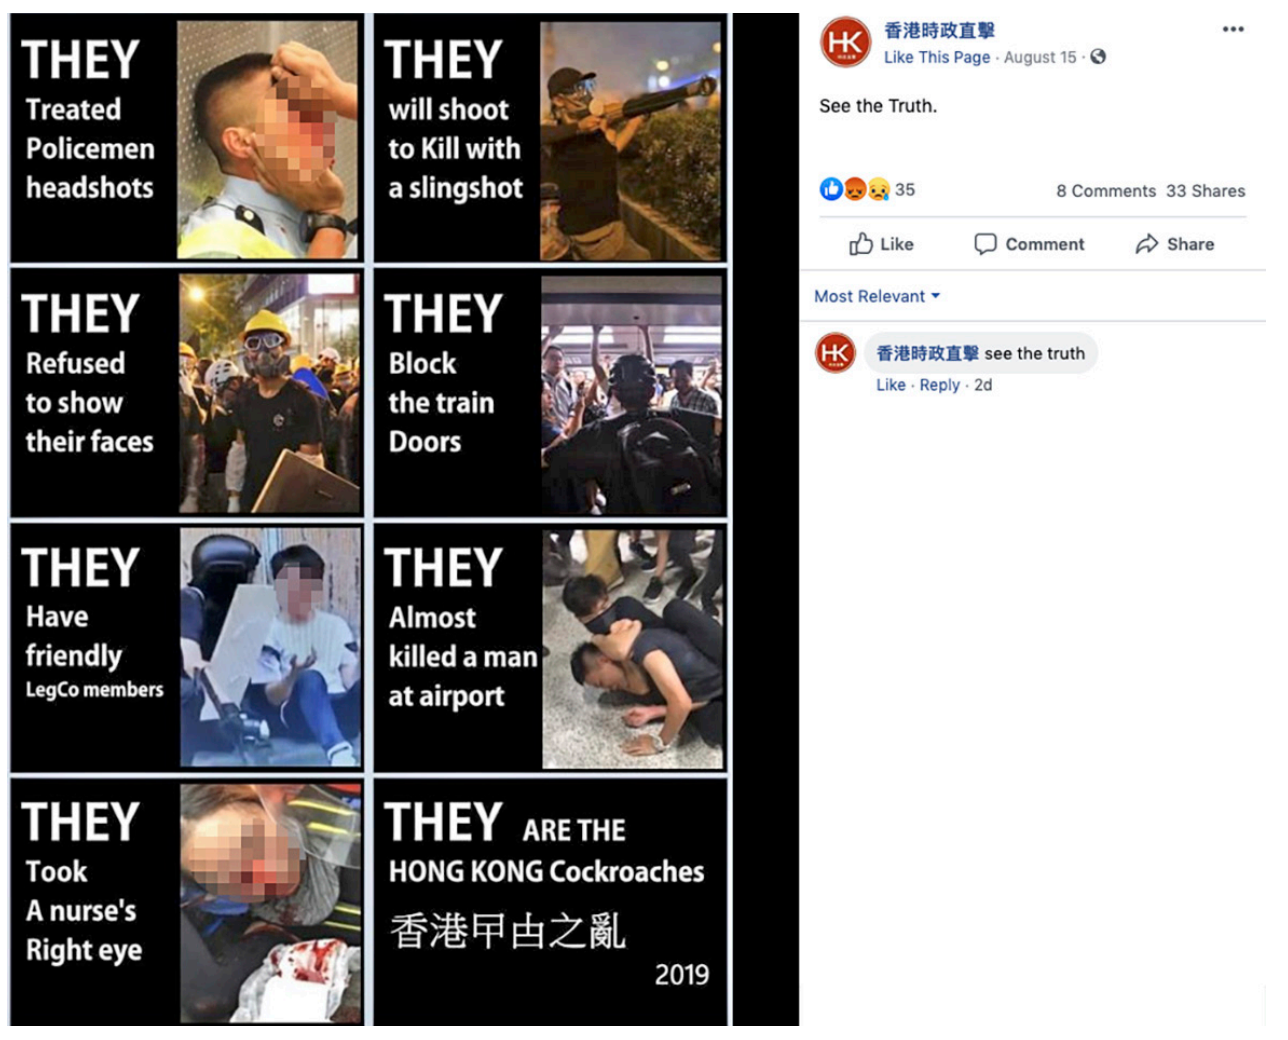
\includegraphics[width=0.9\textwidth]{govt-sponsored-disinfo-3}
            \tiny
            Chinese-sponsored accounts purporting to correct the record of what happened on the ground in Hong Kong
    \end{columns}
\end{frame}

\begin{frame}{Gov-Sponsored Disinfo in Cameroon: \textbf{Real is Fake!}}
    \begin{columns}
        \column{0.5\textwidth}
            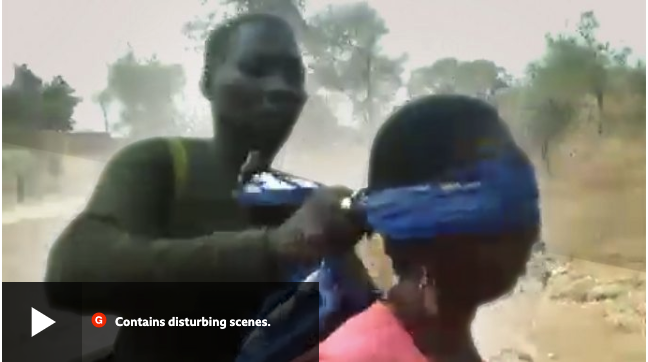
\includegraphics[width=\textwidth]{cameroon-disinfo-1}
            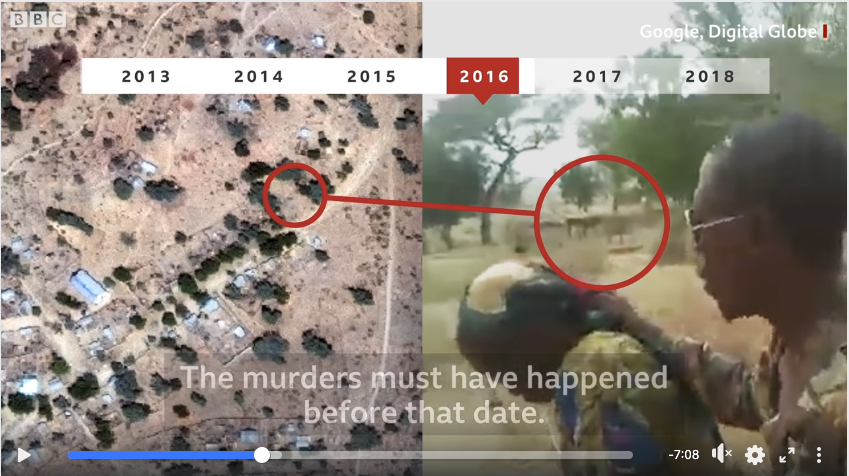
\includegraphics[width=\textwidth]{cameroon-disinfo-2}
        \column{0.5\textwidth}
            \begin{itemize}
                \item Two Anglophone Cameroonian women killed by security forces with babies still on their backs for their alleged participation in Boko Haram.
                \item Video went viral on social media.
                \item Gov. dismissed as “fake news”.
                \item Carefully researched BBC investigation confirmed video veracity, location in Cameroon, and perpetrators part of Cameroon’s security forces.
            \end{itemize}
    \end{columns}
\end{frame}

\begin{frame}{Gov-Sponsored Disinfo in Cameroon: \textbf{Fake is Real!}}
    \begin{columns}
        \column{0.5\textwidth}
            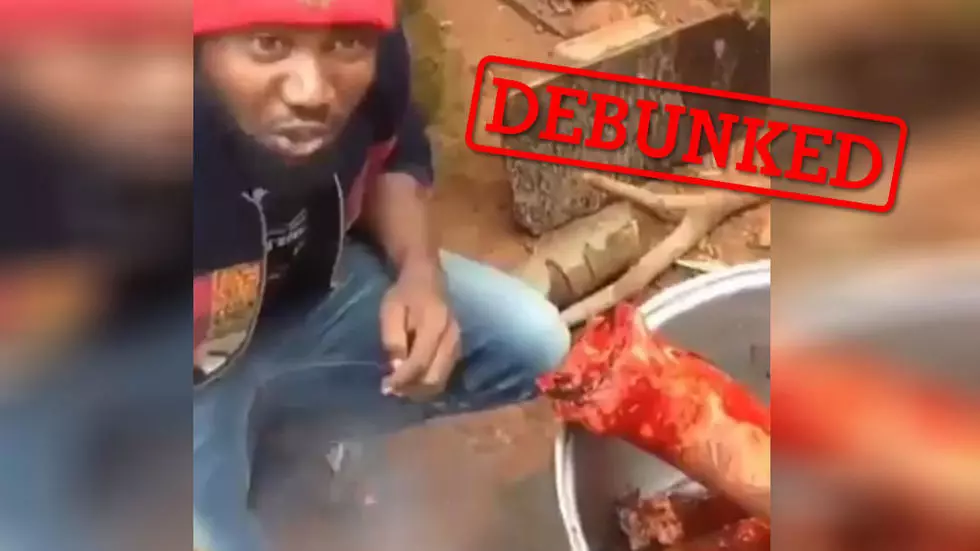
\includegraphics[width=\textwidth]{cameroon-disinfo-3}
        \column{0.5\textwidth}
            \begin{itemize}
                \small
                \item Facebook video showed a man cooking human body parts in a pot over a wood fire.
                \item Video went viral, with many claiming that the video was shot in the Anglophone region.
                \item In fact, the video was created by a Nigerian make-up artist, Hakeem Onilogbo.
                \item Five days after the post, Cameroon’s government used the video to justify an army clampdown against the Anglophones, claiming in a widely broadcast statement that “Boko Haram committed atrocities, but they did not cut up humans and cook them in pots.”
            \end{itemize}
    \end{columns}
\end{frame}

\begin{frame}{Information Operations in Support of Private Interests}
    \begin{columns}
        \column{0.6\textwidth}
            \centering
            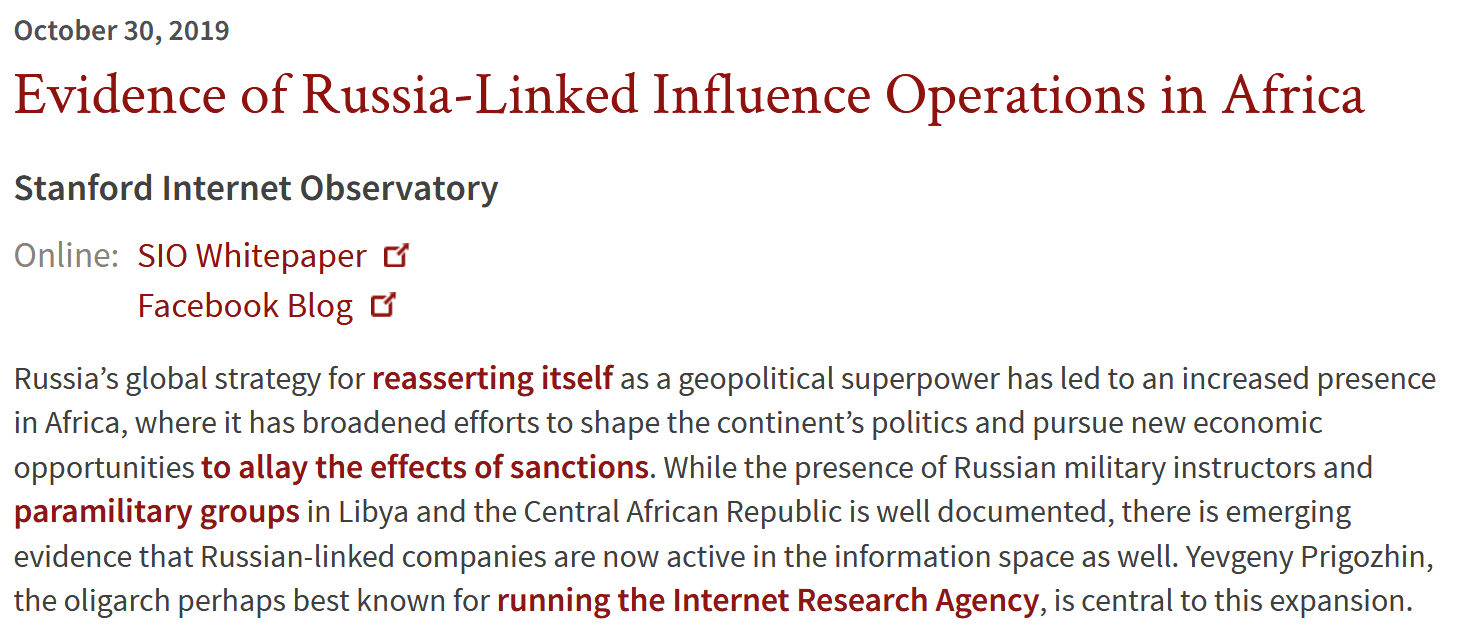
\includegraphics[width=\textwidth]{private-info-ops-1}
            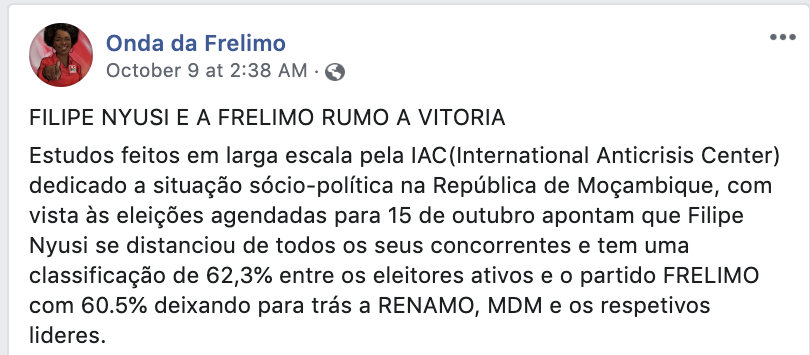
\includegraphics[width=0.8\textwidth]{private-info-ops-2}
        \column{0.4\textwidth}
            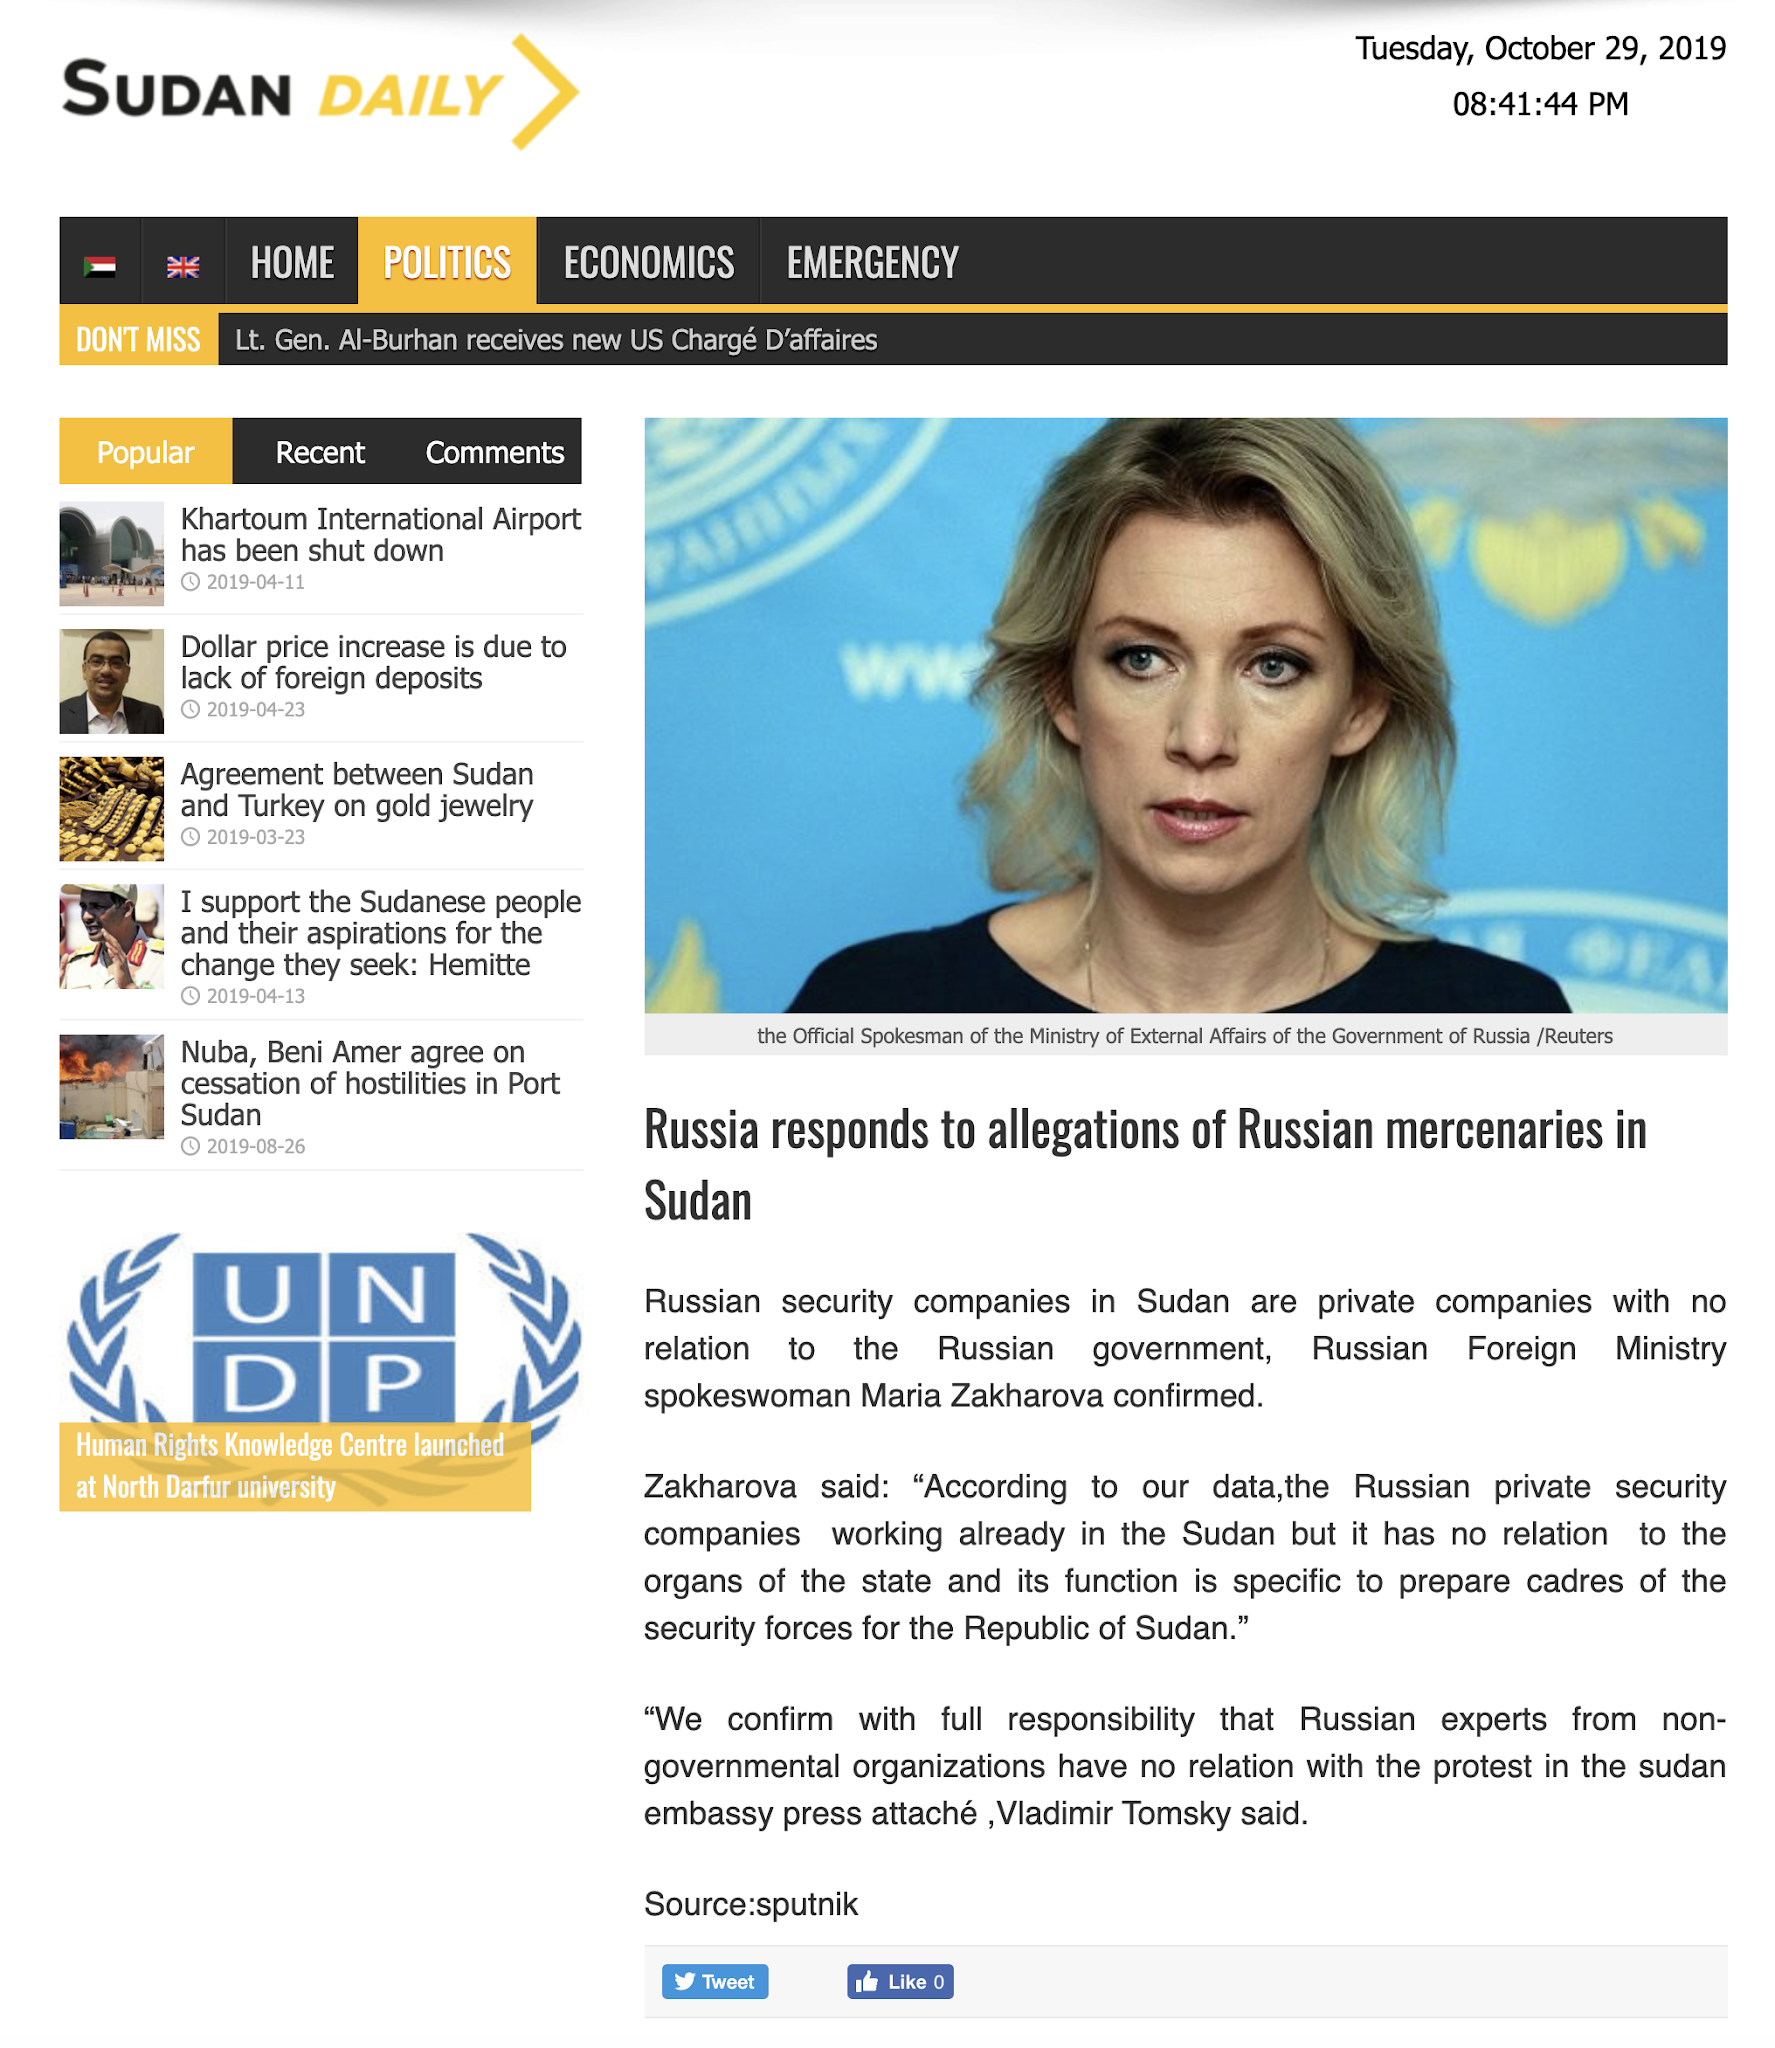
\includegraphics[width=\textwidth]{private-info-ops-3}
    \end{columns}
\end{frame}

\begin{frame}{Political Propaganda}
    \begin{columns}
        \column{0.7\textwidth}
            \begin{itemize}
                \item Propaganda is information with an agenda
                \begin{itemize}
                    \item It’s intended to be emotionally resonant 
                    \item It often contains some degree of factually accurate information, making it difficult to dispute
                    \item It’s inflected to appeal to a particular point of view
                \end{itemize}
                \item It is a very, very old tactic  
            \end{itemize}
        \column{0.3\textwidth}
            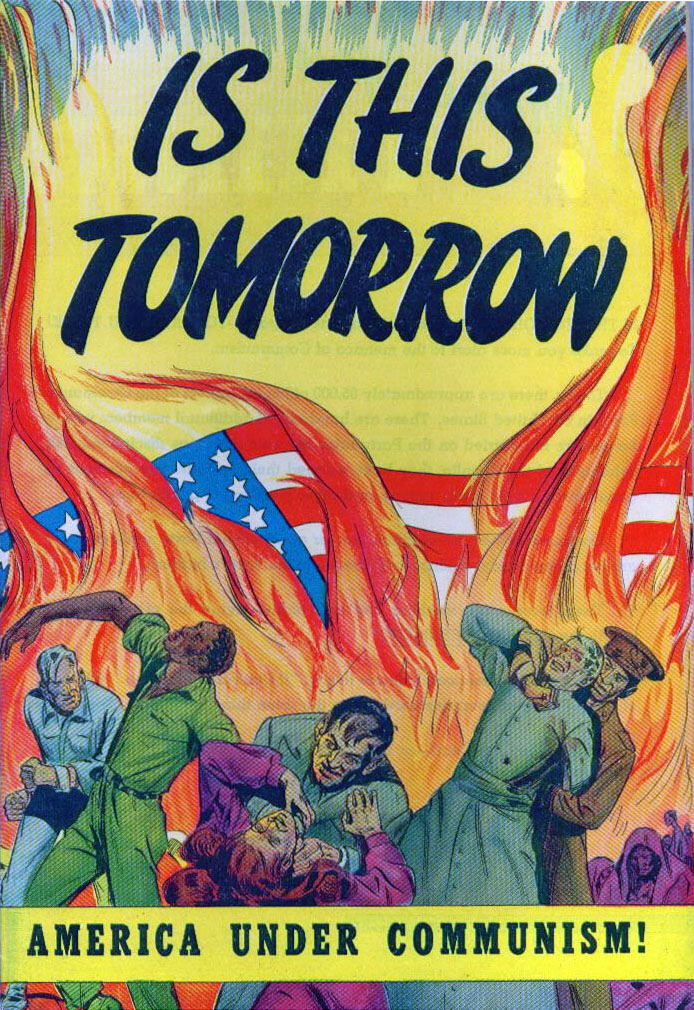
\includegraphics[width=\textwidth]{is-this-tomorrow}
    \end{columns}
\end{frame}

\begin{frame}{Fake News (and why we won't be using this term again)}
    \begin{columns}
        \column{0.4\textwidth}
            Fake news did not originally mean “things I don’t like on the Internet.”  It referred to demonstrably, provably false stories - things that never happened.\\~\\
            
            Fake news, also a significant issue in 2015-2016, is also not a new problem.
        \column{0.6\textwidth}
            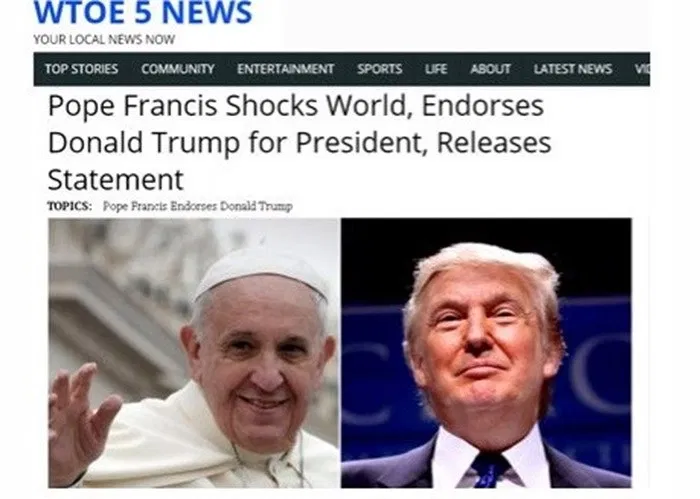
\includegraphics[width=0.9\textwidth]{pope-endorses-trump-fake}
            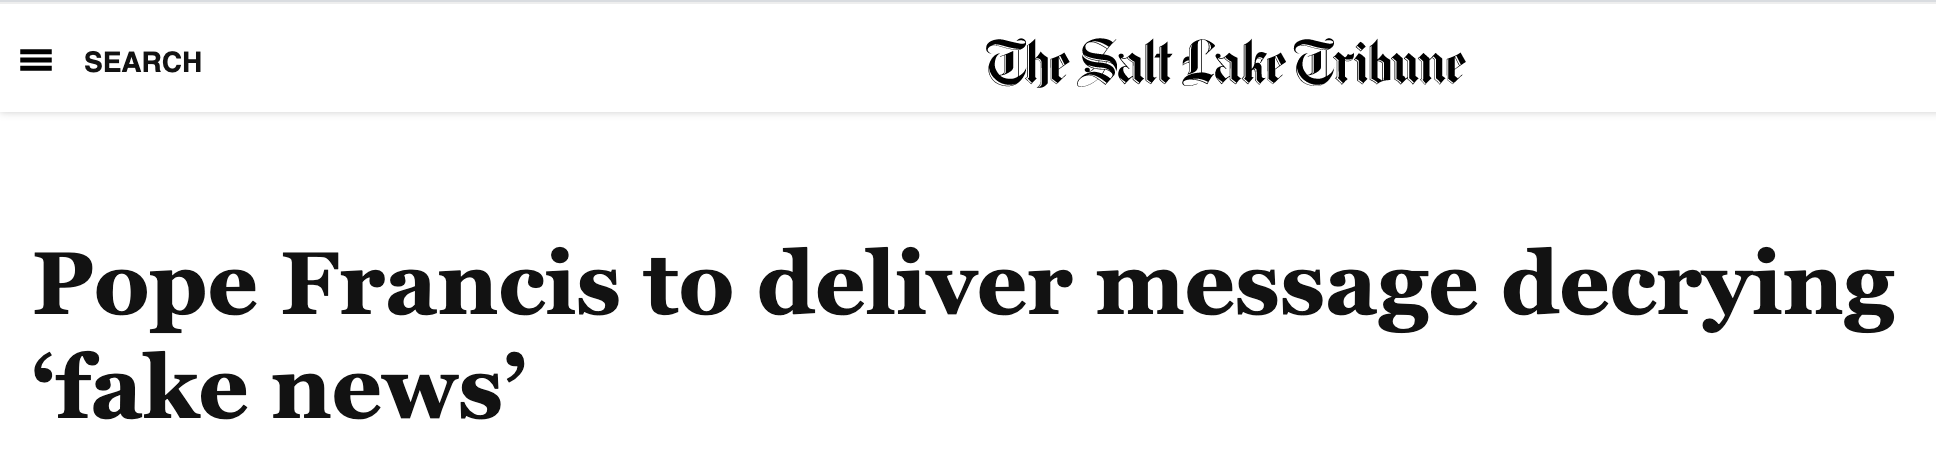
\includegraphics[width=\textwidth]{pope-decries-fake-news}
    \end{columns}
\end{frame}

\begin{frame}{What Makes Active Measures "Active?"}
    \begin{columns}
        \column{0.3\textwidth}
            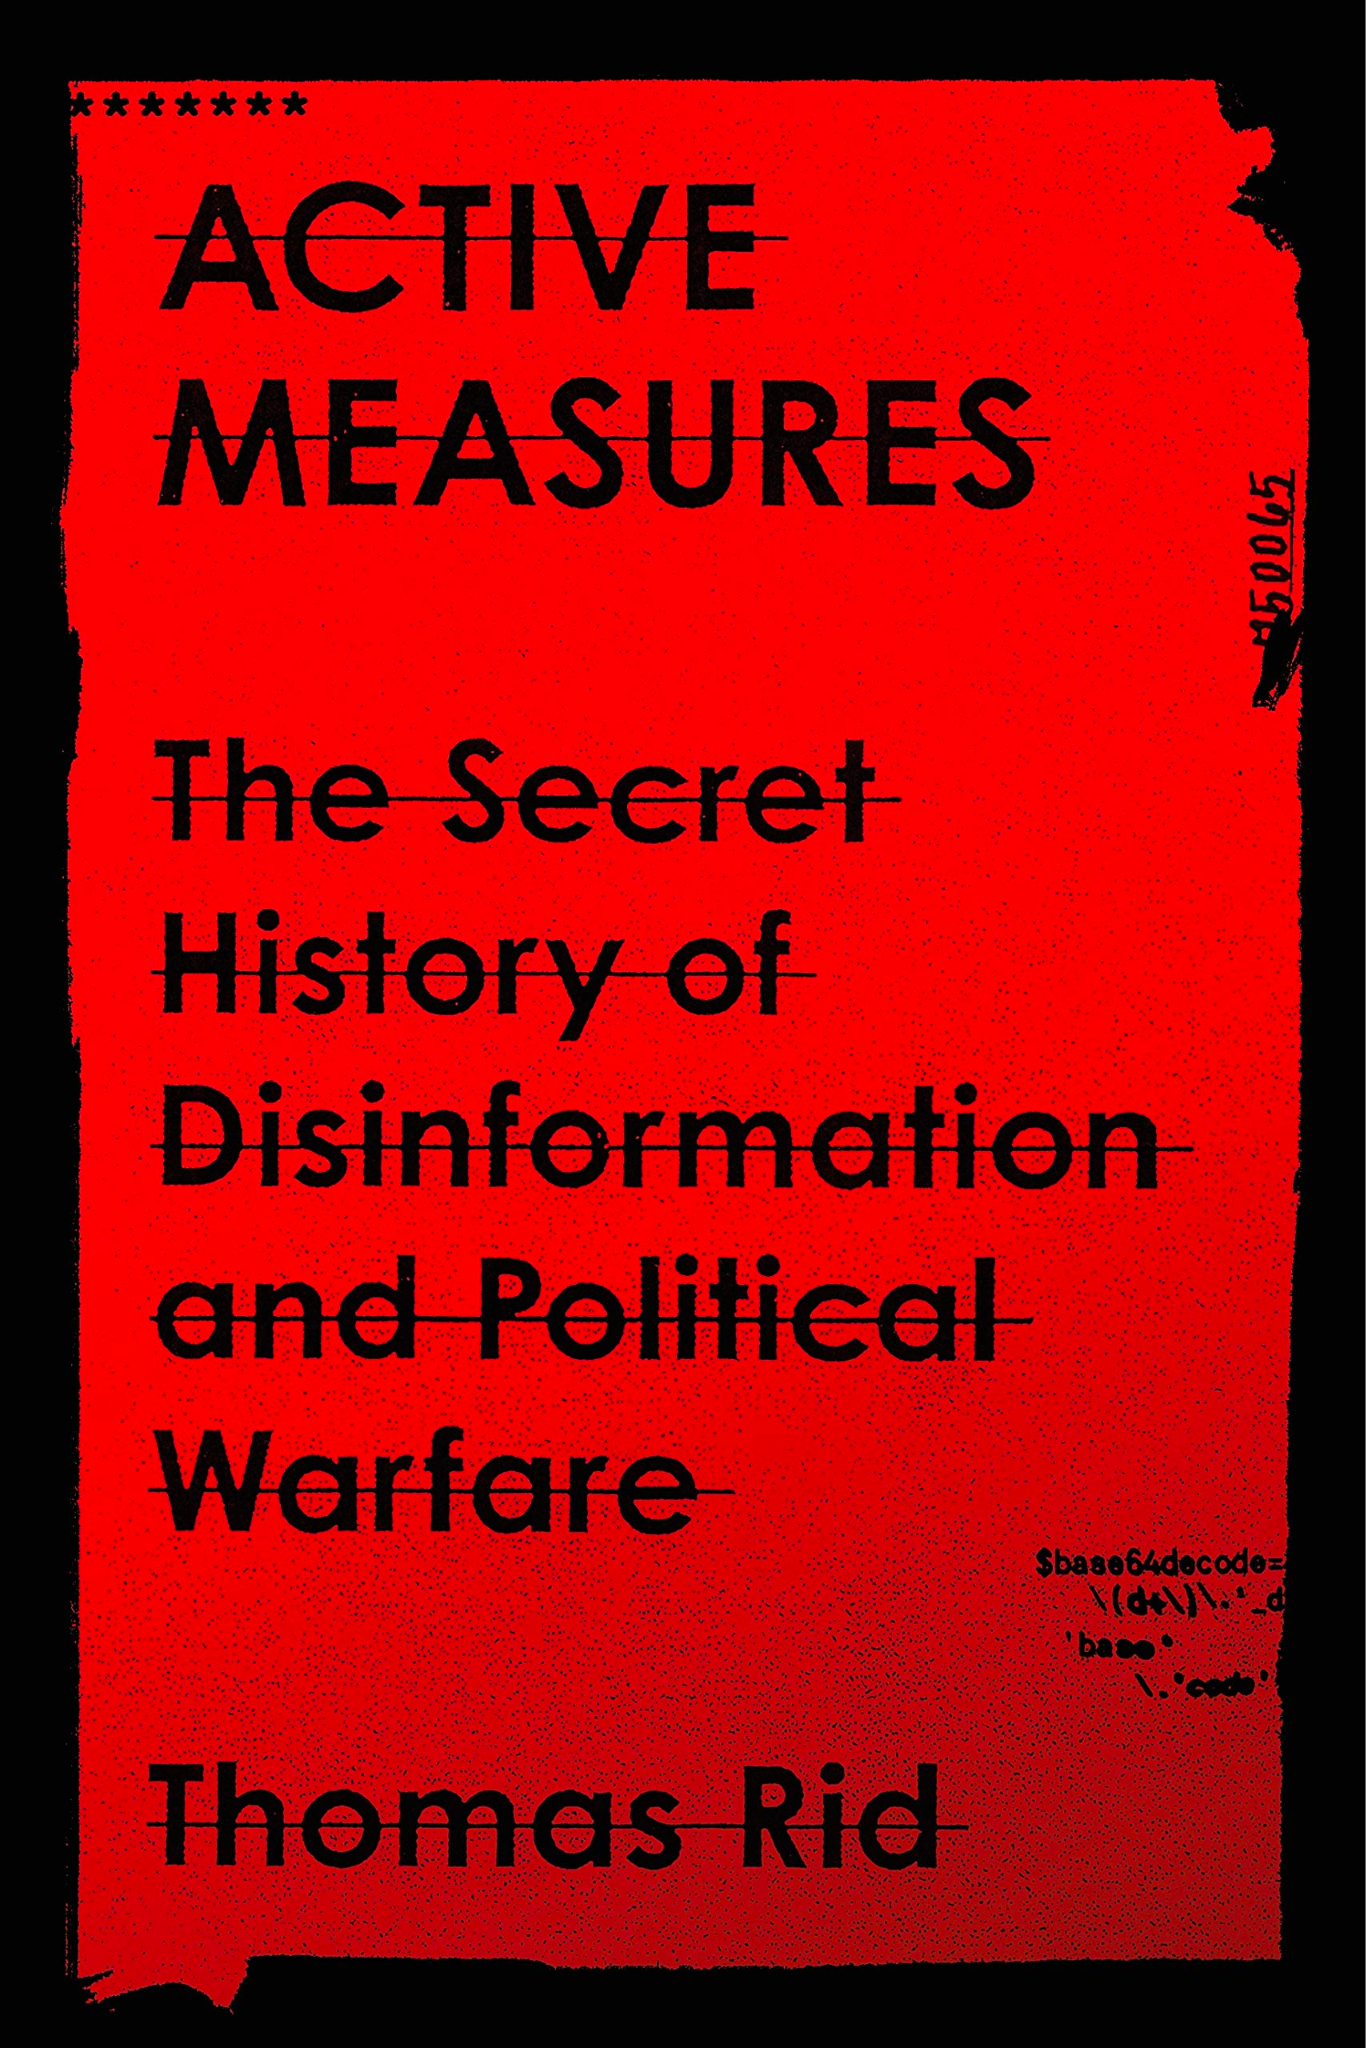
\includegraphics[width=\textwidth]{active-measures}
        \column{0.7\textwidth}
            \href{https://youtu.be/tnyKgVpLcAM}{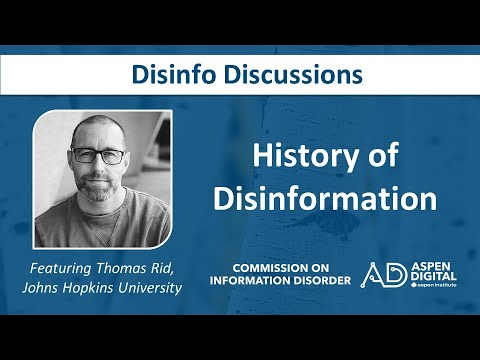
\includegraphics[width=\textwidth]{active-measures-vid}}
    \end{columns}
\end{frame}

\section{Amplification of Information Disorder and Its Effects}

\begin{frame}{Role of Social Media}
    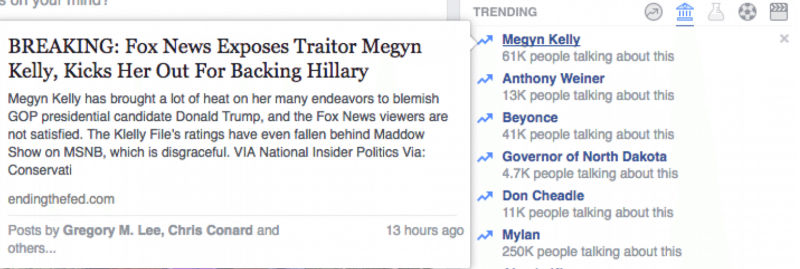
\includegraphics[width=\textwidth]{role-of-social-media}
\end{frame}

\begin{frame}{Disinformation Kill Chain}
    \begin{columns}
        \column{0.5\textwidth}
            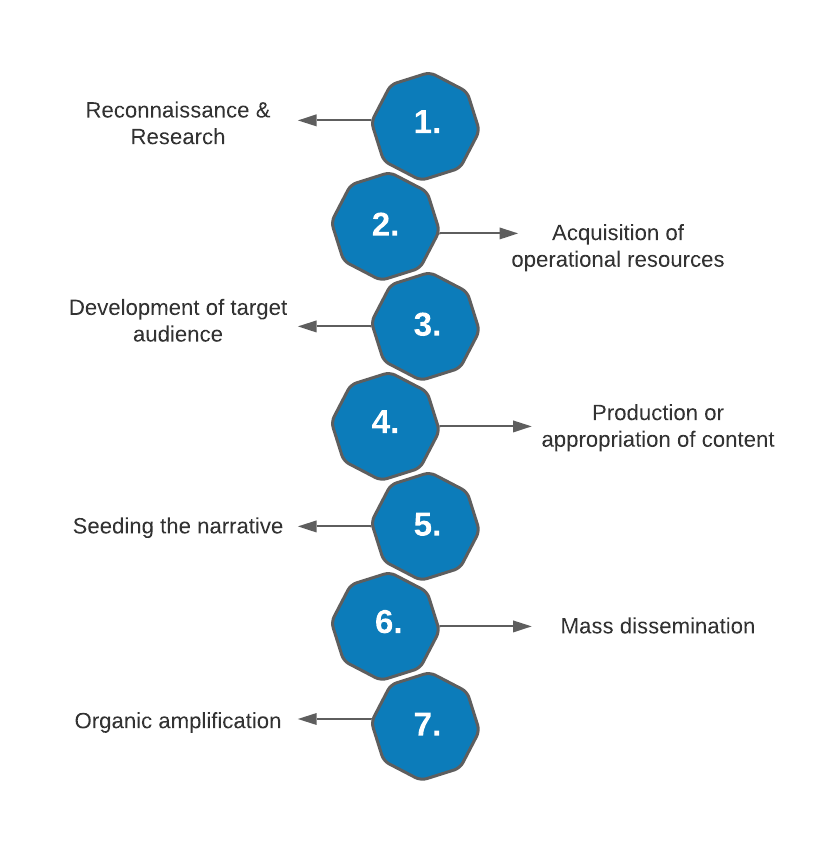
\includegraphics[width=\textwidth]{disinfo-kill-chain}
        \column{0.5\textwidth}
            \begin{enumerate}
                \item Reconnaissance \& research
                \item Acquisition of operational resources
                \item Development of target audience
                \item Production or appropriation of content
                \item Seeding the narrative
                \item Mass dissemination 
                \item Organic amplification
            \end{enumerate}
    \end{columns}
\end{frame}

\begin{frame}{The Trumpet of Amplification}
    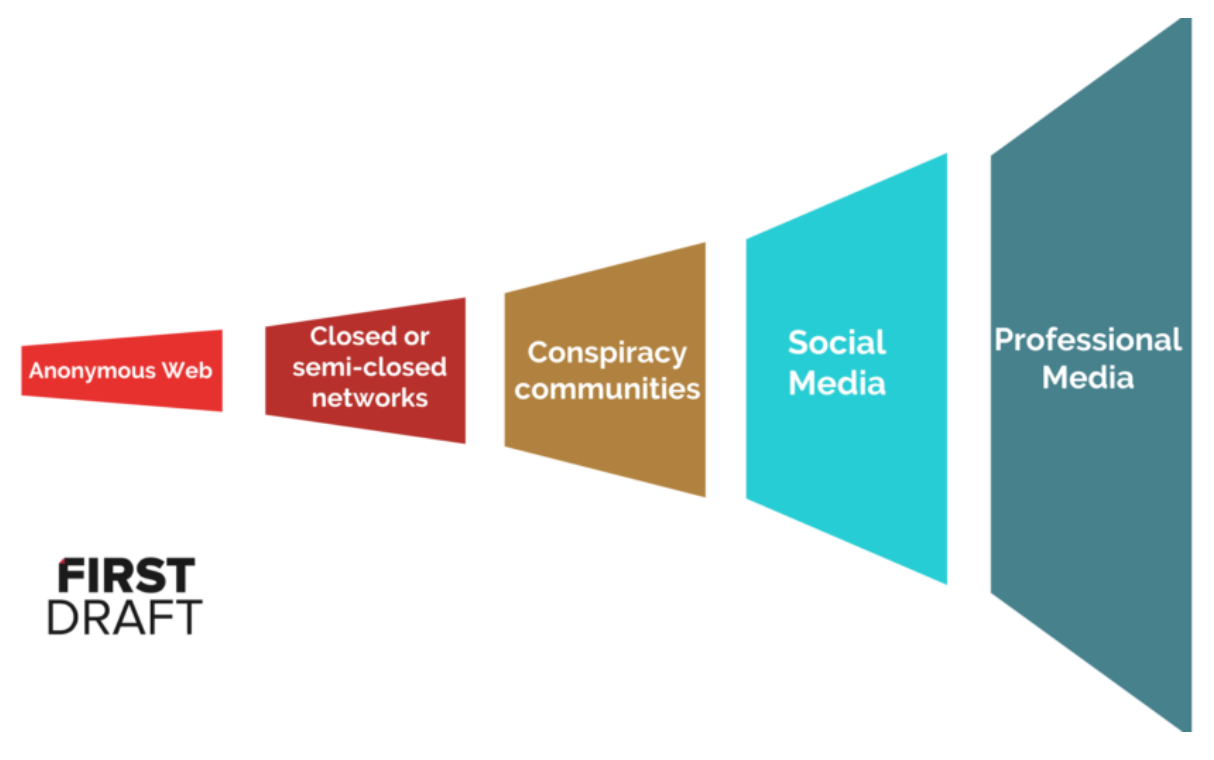
\includegraphics[width=0.9\textwidth]{amplification-trumpet}
\end{frame}

\section{Responses and Mitigations}

\begin{frame}{Policy Responses}
    \large
    \begin{itemize}
        \item Build out new platform policy regimes
        \item Increase transparency, including clear definitions
        \item Share research about misinformation
        \item Support for immune system (fact-checking efforts, media literacy training programs, and funding research)
        \item Inform debates about legislation
        \item Hire politically-neutral regional and local experts
    \end{itemize}
\end{frame}

\begin{frame}{Major Policy Breakdown}
    \centering
    \LARGE
    Actor\\
    or\\
    Content?
\end{frame}

\begin{frame}{\#WarOnPineapple}
    \centering
    \begin{columns}
        \column{0.5\textwidth}
            \centering
            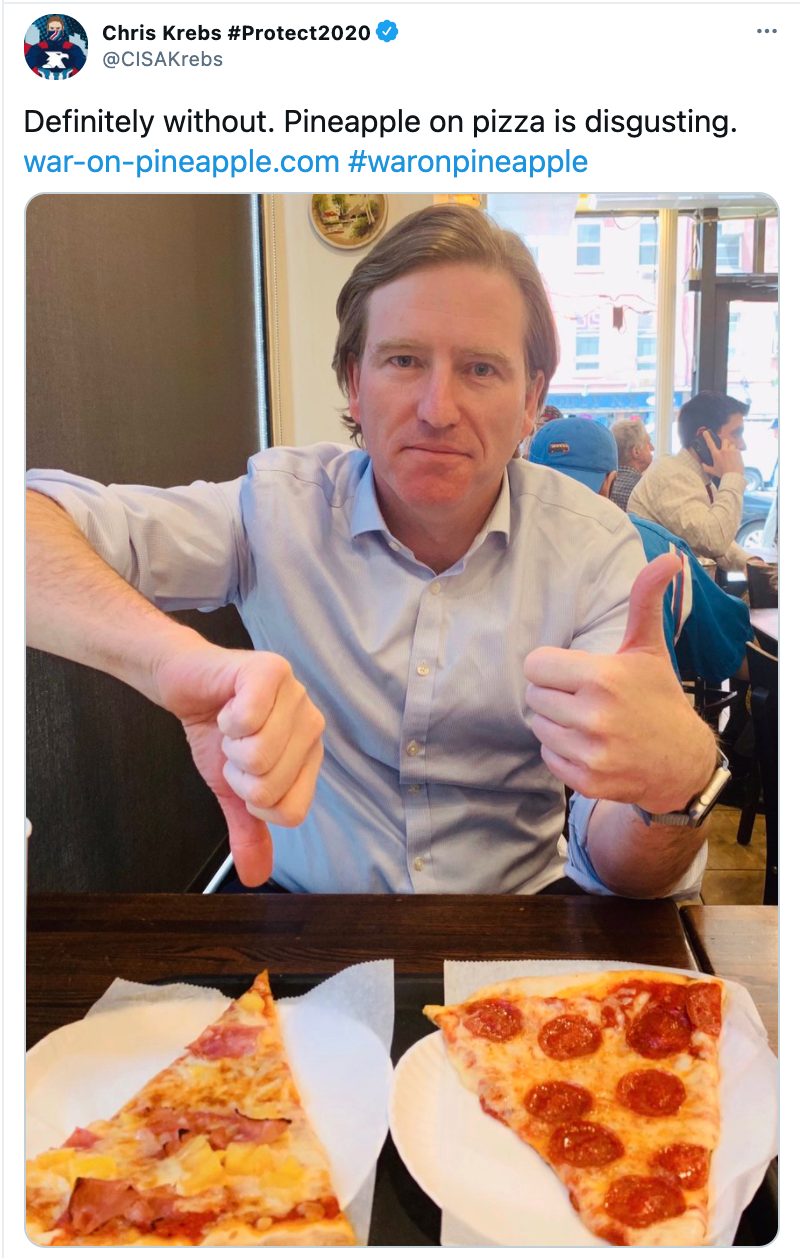
\includegraphics[width=0.7\textwidth]{waronpineapple-1}
        \column{0.5\textwidth}
            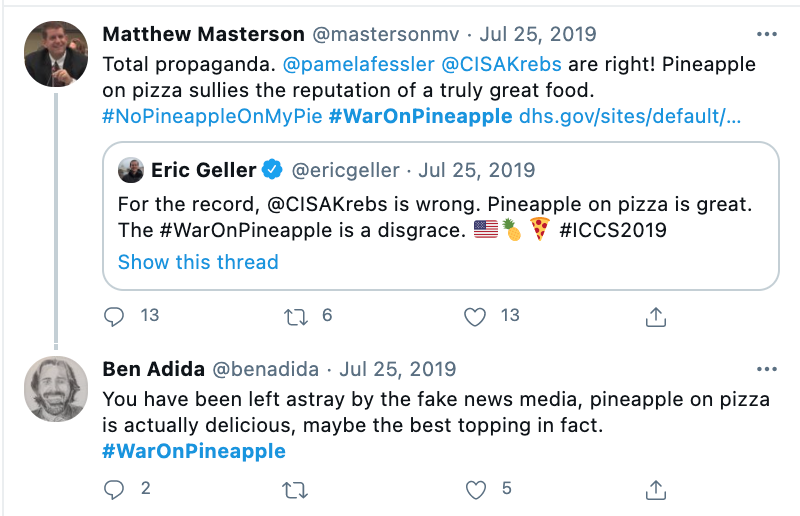
\includegraphics[width=\textwidth]{waronpineapple-2}
    \end{columns}
\end{frame}

\begin{frame}{\#WarOnPineapple}
    \begin{columns}
        \column{0.6\textwidth}
            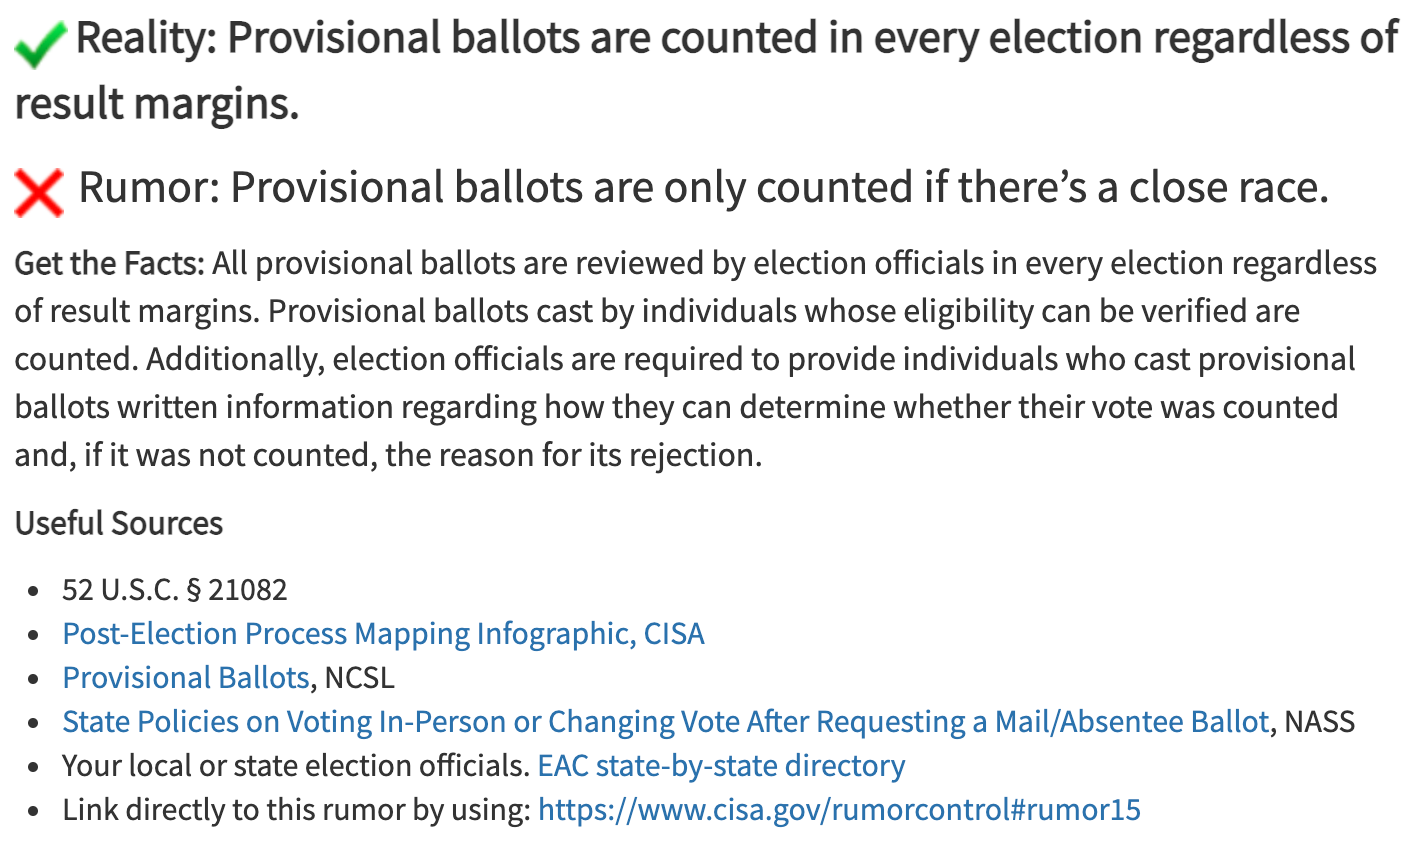
\includegraphics[width=\textwidth]{waronpineapple-3}
        \column{0.4\textwidth}
            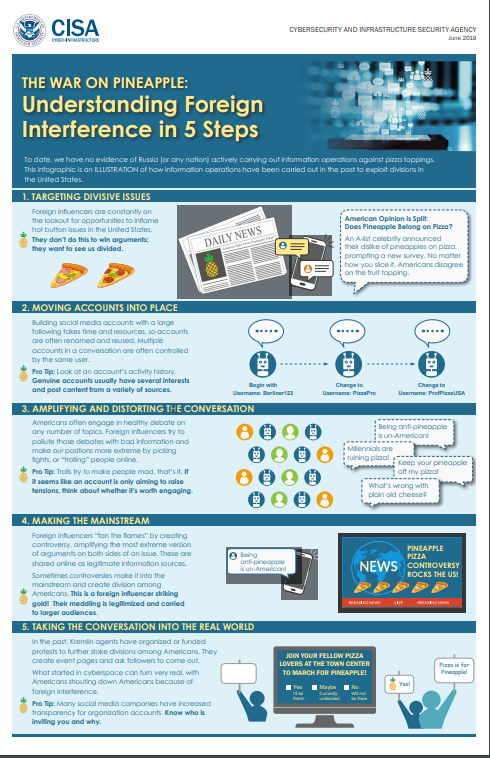
\includegraphics[width=0.9\textwidth]{waronpineapple-4}
    \end{columns}
\end{frame}

\begin{frame}{Product and Technical Responses}
    \large
    \begin{itemize}
        \item Reduce maximum velocity, virality and volume through friction
        \item Reduce the financial incentives for disinformation
        \item Label potential misinformation and disinformation
        \item Treat influencers differently
        \item Build machine learning classifiers
        \item Protecting highly targeted individuals
    \end{itemize}
\end{frame}

\begin{frame}{Labeling Content}
    \begin{columns}
        \column{0.4\textwidth}
            
\includegraphics[width=\textwidth]{labeling-content-search}
        \column{0.6\textwidth}
            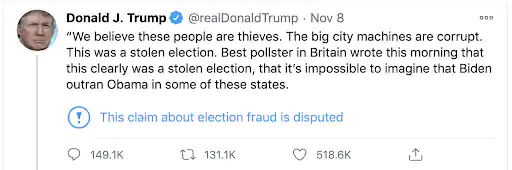
\includegraphics[width=\textwidth]{labeling-content-trump-1}
            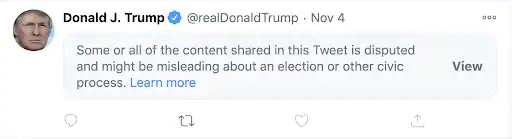
\includegraphics[width=\textwidth]{labeling-content-trump-2}
    \end{columns}
\end{frame}

\begin{frame}{Are Labels Effective?}
    Take a minute and brainstorm with one or two other people: Why might labels be effective? What might be some unintended consequences?\\~\\
    \begin{itemize}
        \item Labeling content as “disputed” or “rated false” lowers perceived accuracy of headline (Clayton et al 2019 - MTurk experiment; fairly robust finding)
        \item This effect also holds for accurate headlines (Freeze et al 2021- MTurk experiment)
        \item “Implied truth effect” where unlabeled content must be true (Pennycook et al 2020- MTurk experiment)
        \item What about the “backfire effect”? Little evidence that it’s robust. (Nyhan 2019)
    \end{itemize}
    General critique: Reliance on online surveys. Why might this be a problem?
\end{frame}

\begin{frame}{Need Research into Effect of (Very Common) Generic Labels}
    \centering
    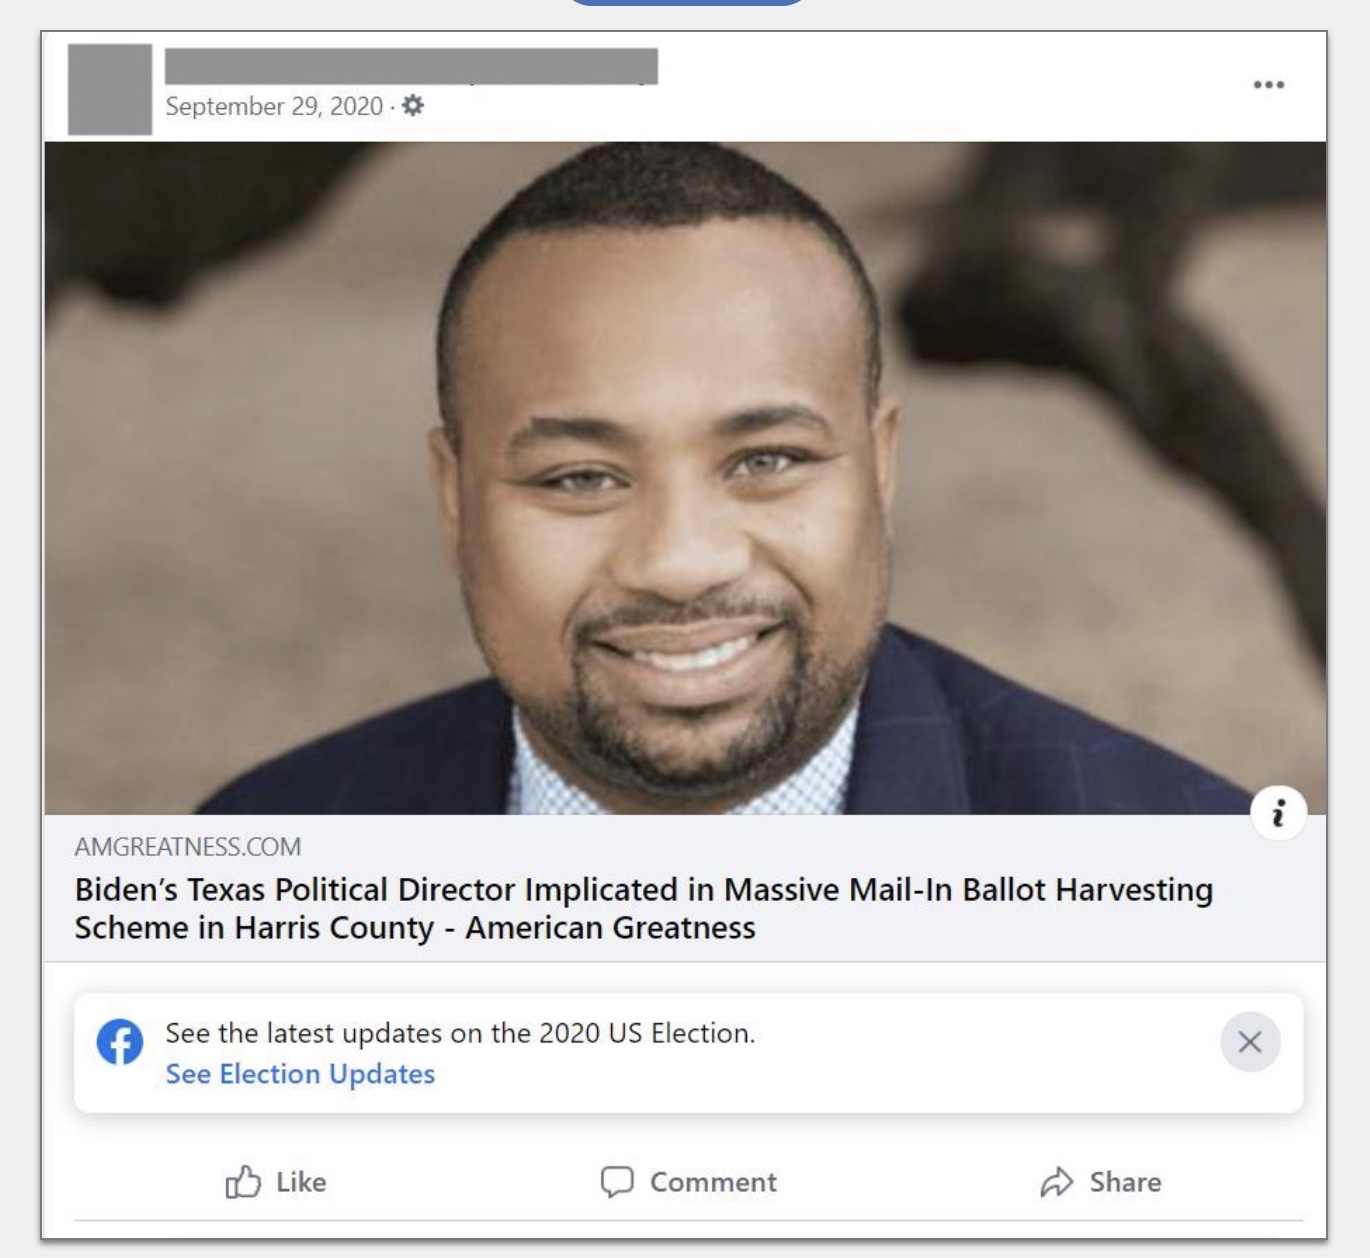
\includegraphics[width=0.6\textwidth]{labeling-impact}
\end{frame}

\begin{frame}{What Can We Do in Free Societies?}
    \centering
    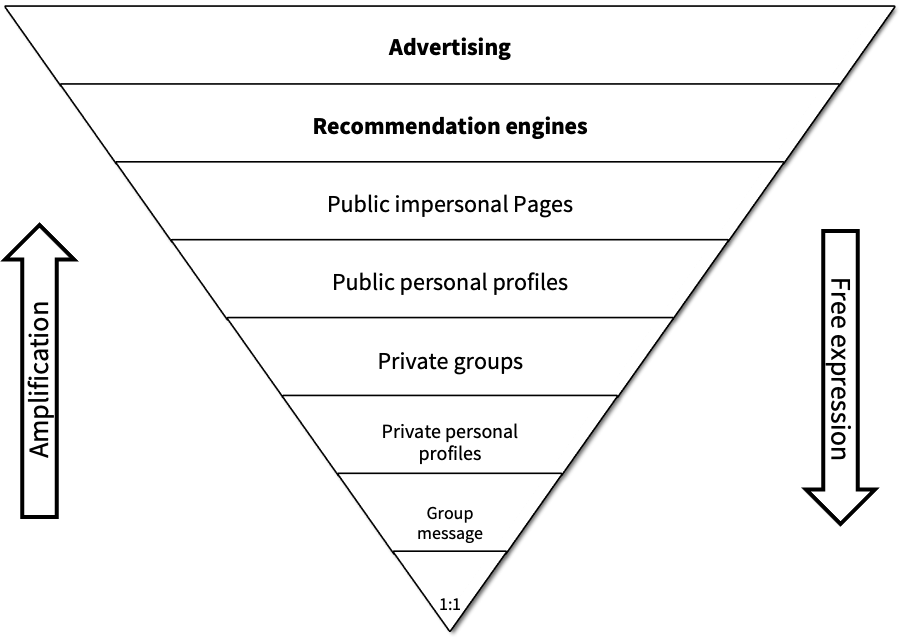
\includegraphics[width=0.8\textwidth]{amplification-pyramid}
\end{frame}

\begin{frame}{What Can We Do in Free Societies?}
    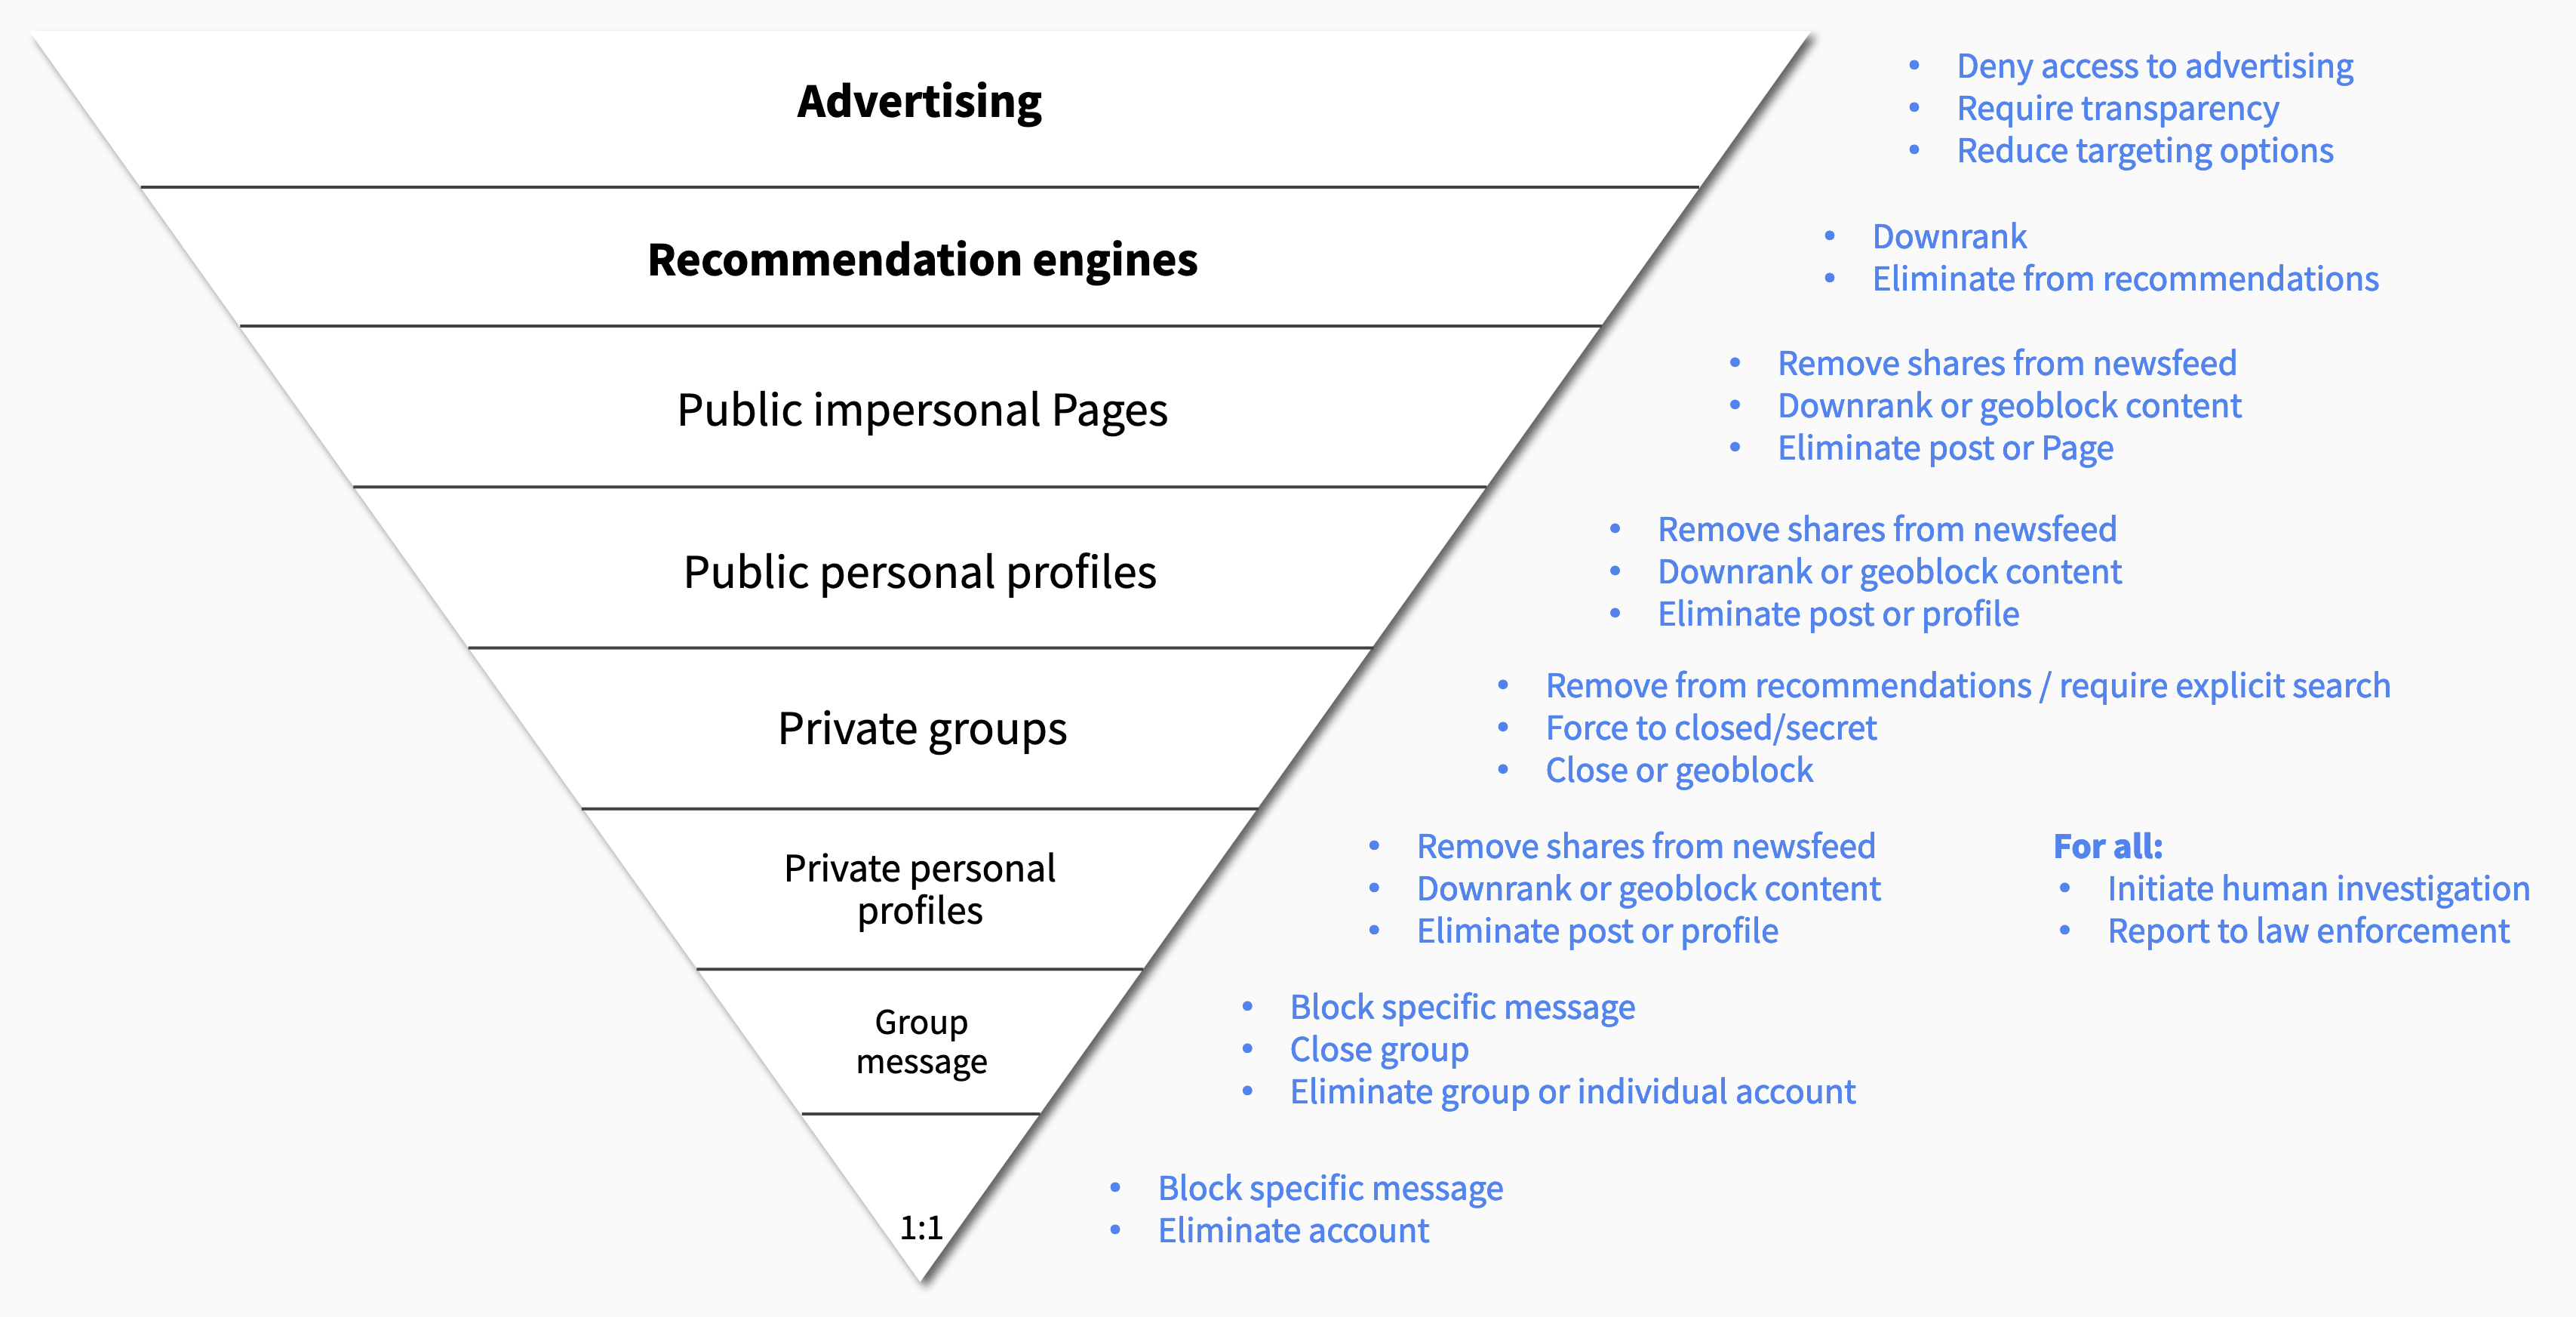
\includegraphics[width=\textwidth]{amplification-pyramid-policies}
\end{frame}

\begin{frame}{Where Is This Going?}
    \large
    \begin{itemize}
        \item Gray-area influence operations
        \item More diversity among actors
        \item Weaponized uncertainty
        \item Use of deepfakes and inauthentic content
        \item E2E
    \end{itemize}
\end{frame}

\section{Discussion}

\begin{frame}{Discussion}
    If you worked at a platform, how would you evaluate the effectiveness of labeling misinformation?\\~\\

    How should a social media platform handle unfalsifiable friend of friend stories, like “My friend’s aunt died from the COVID-19 vaccine. She got vaccinated, and two days later she died”?
\end{frame}
\end{document}